% STEP 1: Choose oneside or twoside. Use the 'draft' option a lot when writing.
\documentclass[english, oneside]{HYgradu}

\usepackage[utf8]{inputenc} % For UTF8 support. Use UTF8 when saving your file.
\usepackage{lmodern} % Font package
\usepackage{textcomp}
\usepackage[pdftex]{color, graphicx} % For pdf output and jpg/png graphics
\usepackage[pdftex, plainpages=false]{hyperref} % For hyperlinks and pdf metadata
\usepackage{fancyhdr} % For nicer page headers
%\usepackage{tikz} % For making vector graphics (hard to learn but powerful)
%\usepackage{wrapfig} % For nice text-wrapping figures (use at own discretion)
\usepackage{amsmath, amssymb} % For better math
\usepackage[round]{natbib} % For bibliography
\usepackage[footnotesize,bf]{caption} % For more control over figure captions
\usepackage{subcaption}
\usepackage{arydshln}

\fussy % Probably not needed but you never know...


% OPTIONAL STEP: Set up properties and metadata for the pdf file that pdfLaTeX makes.
% But you don't really need to do this unless you want to.
\hypersetup{
    bookmarks=true,         % show bookmarks bar first?
    unicode=true,           % to show non-Latin characters in Acrobat’s bookmarks
    pdftoolbar=true,        % show Acrobat’s toolbar?
    pdfmenubar=true,        % show Acrobat’s menu?
    pdffitwindow=false,     % window fit to page when opened
    pdfstartview={FitH},    % fits the width of the page to the window
    pdftitle={},            % title
    pdfauthor={},           % author
    pdfsubject={},          % subject of the document
    pdfcreator={},          % creator of the document
    pdfproducer={pdfLaTeX}, % producer of the document
    pdfkeywords={something} {something else}, % list of keywords for
    pdfnewwindow=true,      % links in new window
    colorlinks=true,        % false: boxed links; true: colored links
    linkcolor=black,        % color of internal links
    citecolor=black,        % color of links to bibliography
    filecolor=magenta,      % color of file links
    urlcolor=cyan           % color of external links
}

% STEP 2:
% Set up all the information for the title page and the abstract form.
% Replace parameters with your information.
\title{Formation of cores by merging supermassive black holes}
\author{Joonas Suortti}
\date{\today}
\level{Master's thesis}
\faculty{Faculty of Whatever}
\department{Department of Something}
\address{PL 42 (Kuvitteellinen katu 1)\\00014 Helsingin yliopisto}
\subject{Your Field}
\prof{prof. Smith}
\censors{prof. Smith}{doc. Smythe}{}
\depositeplace{}
\additionalinformation{}
\numberofpagesinformation{\numberofpages\ pages}
\classification{}
\keywords{Your keywords here}
\quoting{``Bachelor's degrees make pretty good placemats if you get them laminated.'' \\---Jeph Jacques}

\begin{document}

% Generate title page.
\maketitle

%\onehalfspacing
\doublespacing

% STEP 3:
% Write your abstract (of course you really do this last).
% You can make several abstract pages (if you want it in different languages),
% but you should also then redefine some of the above parameters in the proper
% language as well, in between the abstract definitions.
\begin{abstract}
Abstract goes here.
\end{abstract}

% Place ToC
\mytableofcontents



% -----------------------------------------------------------------------------------
% STEP 4: Write the thesis.
% Your actual text starts here. You shouldn't mess with the code above the line except
% to change the parameters. Removing the abstract and ToC commands will mess up stuff.
\chapter{Introduction}

\chapter{Background Theory}

\textit{\textbf{Topics that need to be explained for Chapter 4:}
\\
Poisson equation, phase-space, gravitational sphere-of-influence, loss-cone, modified gaussian and hermite polynomials and $h_3$ $h_4$, ellipticity...}

\textit{\textbf{Additional stuff from Chapter 4:}
\\
hard binary, maximum velocity at which stars can interact with loss cone, slow and fast rotator galaxies}

\section{Early-Type Galaxies}

The term "early-type galaxy" (ETG) is used to denote galaxies located on the left-side of  the Hubble sequence \citep[defined by][]{Hubble1926}; a system of morphological classification for galaxies, where they are divided into roughly three categories: elliptical, spiral and irregular galaxies. ETGs consist of the aforementioned elliptical as well as the so-called lenticular galaxies, the latter of which are transitional objects with features from both elliptical and spiral galaxies \citep{BinneyTremaine}, which include a small or non-existent amount of cool gas (and thus a negligible amount of star-formation) as well as having a smooth and relatively featureless appearance. However, whereas lenticular galaxies, like spirals, contain a rapidly rotating disk alongside a central bulge; elliptical galaxies are disk-less and generally more ellipsoidal in their shape, with constant luminosity contours (i.e. isophotes) that can be described as co-centric ellipses \citep{BinneyTremaine}.

Elliptical galaxies are further divided into seven different subcategories according to their ellipticity (E0 - E7; where the number denotes the tenth multiple of the value of the ellipticity rounded to the nearest integer). Ellipticity itself is simply the measure of how flattened an observed 2D-projection of a spherical stellar system is, and can be calculated as:
\begin{equation}
\epsilon = 1 - \frac{b}{a},
\end{equation}
where $a$ and $b$ are the semi-major and semi-minor axes of a luminosity isophote respectively, and where the value of the ellipticity grows alongside the flatness of the system ($\epsilon = 0$ denoting a completely spherical galaxy). It is important to note, however, that the ellipticity of a system depends on the luminosity contour from which it is calculated. As the isophotes of elliptical galaxies generally become flatter farther from its centre \citep{BinneyTremaine}, this could result in a single galaxy having multiple ellipticities. To remedy this, the Hubble classification uses the ellipticity at the effective radius ($R_e$), i.e. the radius which encloses half of the galaxy's luminosity, when determining its elliptical subcategory.

\section{Core and Cusp Galaxies}

As examination of elliptical galaxies (or any extra-galactic object for that matter) consist solely of observations of the light they emit, much of the information about their physical structure comes from the distribution of the observed light. The quantity used for calculating this distribution is the \textit{surface brightness} ($I$), which describes the observed luminosity from a unit area, because astronomical observations are simply two dimensional projections of the actual three dimensional objects. Deriving the distribution of the physical material from the surface brightness distribution is done by applying some mass-to-light ratio ($M/L$) to the surface brightness profile. Assumptions on the $M/L$ can be made if the stellar types in the observed galaxy's population of stars is known. This knowledge can be
gained through, for example, spectral analysis of the chemical composition in the stellar objects.

Since the distribution of surface brightness is an important quantity in studying stellar populations, a multitude of models have been made to describe the general shape of the profiles found commonly in observations. A prominent model used for describing the surface brightness profiles of earl-type galaxies, is the Sérsic-profile \citep{Sersic1968}:
\begin{equation}
I (R) = I_e \exp \{ -b_n \left[ (R / R_e)^{1/n} \right] \},
\end{equation}
where $R$ is the projected distance from the galactic centre, $I_e$ is the surface brightness at the effective radius, $n$ is the so-called Sérsic index, and $b_n$ is a shape factor that is defined so that the definition of $R_e$ hold true. The value for the shape factor can be approximated as $b_n \approx 2n - 0.324$, when $1 \lesssim n \lesssim 10$ \citep{BinneyTremaine}.

The Sérsic model, however, only works well at the outer parts of observed ETGs, as the observed profiles usually diverge from the model's predictions close to the galactic centre \citep{Kormendy2009}. Some galaxies contain "extra" light at short projected distances. These are called \textit{cusp} galaxies, due to the steep cusp-like shape of the inner surface brightness profile. On the other hand, galaxies diverging from the Sérsic profile due to "missing" light are called \textit{core} galaxies. There are a few definitions of what exactly constitutes a core galaxy. \cite{Kormendy1999} define core galaxies as galaxies whose surface brightness profile contains a shallow inner profile and a steep outer profile, whereas \cite{Lauer1995} determine that the surface brightness profile of core galaxies must contain an inner slope of $\gamma < 0.3$. 

This dichotomy between cusp and core galaxies is an important part of ETG research, as although the nomenclature simply refers to the shapes of the surface brightness profiles, both galaxy types show definite differences in both their other photometric properties as well as their kinematics. In general, core galaxies are brighter than cusp galaxies. \cite{GalaxyFormationAndEvo2010} explain that galaxies with magnitudes $\mathcal{M} \lesssim -20.5$ are dominated by core galaxies, where as cusp galaxies dominate the dimmer magnitude range $-20.5 \lesssim \mathcal{M} \lesssim -18$. The rotation of the brighter galaxies is slower than the rotation of the dimmer galaxies, which is connected to core galaxies having boxy isophotes and the cusp galaxies having isophotes that are more disky in shape \citep{Faber1997}. As for the actual velocity distributions, the core galaxies contain relatively anisotropic velocities while showing distinct kinematic structures such as \textit{Kinematically Distinct Cores} (KDC) and kinematic twists, whereas the velocities of cusp galaxies are more isotropic with disk-like kinematics \citep{Kormendy2009, Krajnovic2008}.

\textit{information about sources in notebook}

\section{Core Formation}

\subsection{Black Hole Mergers}

The most prominently proposed mechanism for the formation of the cores seen in massive ETGs, is the ejection of stellar material due to three-body interactions between stars and merging supermassive black holes.

\subsubsection{Merger Event}

\subsubsection{Observations of Binary Black Holes}

\subsection{Other Formation theories}

\section{Galactic Dynamics}

\subsection{Potential Theory}

\subsection{Collisionless Systems}

\subsection{Regularisation}

\subsection{Post-Newtonian Dynamics}

\section{Analysis of the Kinematics in Galaxies}

\chapter{KETJU}

\textit{Description of basic functionality: what KETJU does, why it's created, basic description of the multiple integration region system.} 

\section{AR-CHAIN / Chain Integrator}

\textit{Chain forming, force calculations, integration}

\section{GADGET-3 / Tree Integrator}

\textit{Softening, tree-codes, calculations}

\section{Combined Functionality}

\textit{How the AR-CHAIN and GADGET-3 integrators work together: time-step problem, tidal-perturbations, particles moving from one region to another, chain macro-particle}

\subsection{Particle Types}

\textit{Chain particles, tree particles, perturber particles}

\section{Merging of Black Hole Particles}

Since we are trying to determine if merging SMBH binaries form cores in merger remnants, we must make sure that the progenitors' central black holes actually merge in our simulations. This is done by looking at the "Run" simulations, as they contain the locations of the black holes from multiple time steps, and as the "Snapshots" still show both of the SMBHs.

Plotting the positions of the black holes from "Run 3" in coordinates centred on the binary's centre-of-mass during the initial time step gives us figure \ref{figure:run3_traj}. Even by eye, one can clearly see that the orbit of the black hole with a smaller mass becomes smaller and smaller as the binary moves further away from its initial position. While this doesn't explicitly tell us that the black holes merge into each other, it does indicate the existence of a hardening process in the binary. Similar figures to figure \ref{figure:run3_traj} from all four "Runs" can be found in the appendix (figure \ref{figure:all_traj}).

\begin{figure}[h]
	\centering	
	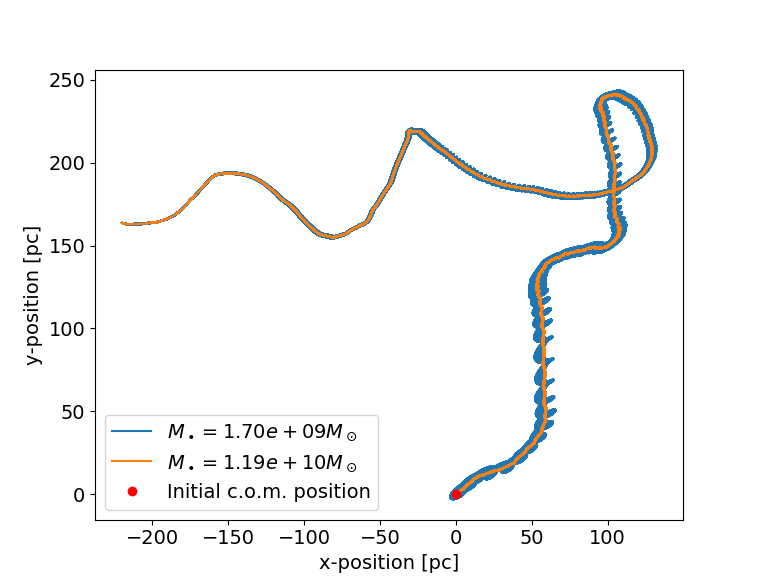
\includegraphics[width=0.7\textwidth]{Run3_Trajectory.png}	
	\caption{The trajectories of the black holes during "Run 3". The coordinates are centred on the initial location of the centre-of-mass of the binary black hole. The orange and blue lines show the paths taken by the smaller and larger black holes respectively. Both paths show clear spiral patterns which become smaller and smaller as the simulation proceeds. The paths end at the location where the black holes merge, i.e. where the distance between them is $\lesssim 100 R_s$ ($R_s$ is the Schwarzschild radius).}
	\label{figure:run3_traj}
\end{figure}

\begin{figure}[h]
	\centering
	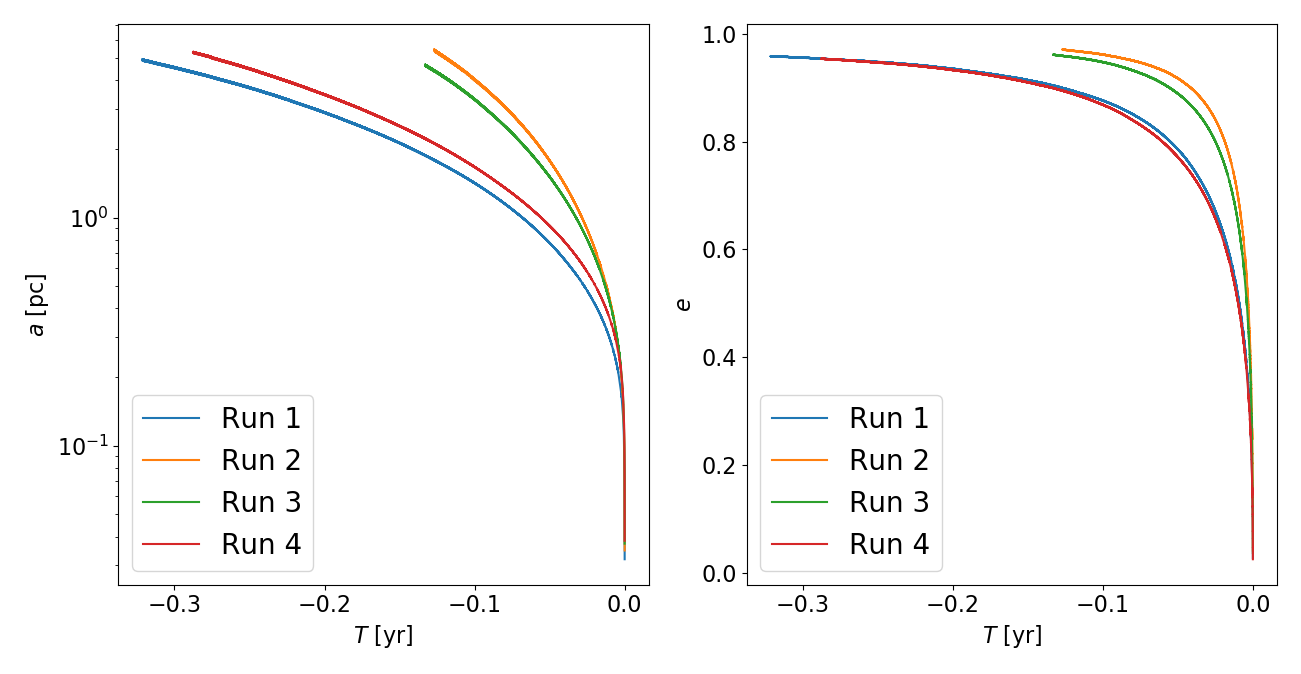
\includegraphics[width=\textwidth]{semi_major_and_ecc.png}
	\caption{The semi-major axes (left) and eccentricities (right) of the black hole systems in the simulations "Runs 1"-"Run-4" as a function of time. The zero position on the x-axis corresponds to the point in simulation time, where the black hole merging event occurs.}
	\label{figure:semi_and_ecc}
\end{figure}

The most likely obstacle for the complete merging of the binary black holes is the so-called final-parsec problem; where, due to the lack of stellar material that can be ejected during the three-body scattering phase, the hardening of the binary stops when the separation between the two black holes is $\sim 1 \mathrm{pc}$. This is assumed to happen since, not only is the binary constantly ejecting the finite amount of stars inside the loss-cone (defined in section 2), but the loss cone itself is becoming smaller due to the contracting binary orbit.

Figure \ref{figure:semi_and_ecc} shows the time evolution of both the semi-major axis and the eccentricity of the binary orbits from all of the simulation runs. Interestingly enough the semi-major axes of all of the binaries go far below single parsec scales, meaning that the final-parsec problem doesn't seem to play a part in the simulations. This implies that, there exists some loss-cone refill mechanism which allows the binary to eject more stellar material than what initially exists inside the loss cone.



\chapter{Merger Simulations Using KETJU}

In this chapter I study the formation of cored galaxies formed in galaxy mergers. The analysis focuses on the results from KETJU simulations run by \cite{Rantala2018}. In all but one simulation, the merger progenitor galaxies contain central supermassive black holes. During the merger event the SMBHs form a hard binary, a likely source for the observed cores, as the binary can eject stars from the galactic centre through complex three-body interactions. Here I determine if there is a connection between the binary SMBH and the existence of a core deficient in light, and if the simulated KETJU results agree with observations of cored galaxies.


\section{Simulation Details}

The simulation sample run by \cite{Rantala2018} includes seven different equal-mass mergers of two identical galaxies. The merger progenitor galaxies (named BH-0 - BH-6) used in the different simulations consist of stellar and dark matter particles, where every stellar particle has an identical mass, as does every dark matter particle. The progenitors are gas free (i.e. the simulations describe so-called "dry" mergers), and all of them but one contains an SMBH at their centre.

The initial conditions (IC) of the merger progenitor galaxies are modelled as multicomponent spherically symmetrical stellar systems, consisting of the three aforementioned components: stellar particles, dark matter particles and a central SMBH. The SMBH components are simply single point masses located at the origin of the galaxies' internal coordinate systems; while the stellar and dark matter components consist of particles which are distributed according to the spherically symmetric Dehnen density-potential model defined as \citep{Dehnen1993}:
\begin{equation}
\rho(r) = \frac{(3-\gamma)M}{4\pi} \frac{a}{r^\gamma (r+a)^{4-\gamma}}, \label{eq:dehnen_density}
\end{equation}
\begin{equation}
\phi(r) = \frac{GM}{a} \times 
\begin{cases}
	-\frac{1}{2-\gamma} \left[ 1 - \left( \frac{r}{r+a} \right)^{2-\gamma} \right] & \; \gamma \neq 2 \\
	\ln \frac{r}{r+a}	 & \; \gamma = 2
\end{cases},
\label{eq:dehnen_potential}
\end{equation}
where $M$ is the total mass, $a$ is a scaling radius, and $\gamma$ is the central slope of the profile. For stellar particles we set $\gamma = 3/2$, while for the dark matter particles the value of $\gamma = 1$ is used. The density profile above is a generalization of stellar density models which, when projected, resemble the de Vaucouleurs - profile \citep[$\log(\mu) \propto R^{1/4}$;][]{deVaucouleurs1948} in the outer parts; while the corresponding gravitational potential profile is derived using the Poisson equation. 

When constructing the multicomponent ICs of the progenitors, the positions of the stellar and dark matter particles are determined through their respective cumulative mass profiles. These are defined using the Dehnen density-potential model, and can be written as:
\begin{equation}
M(r) = 4\pi \int^r_0 \rho(r)r^2 \;dr = M \left( \frac{r}{r+a} \right)^{3-\gamma}, \label{eq:cumulative_mass}
\end{equation}
where $\rho(r)$ is the density profile from equation \ref{eq:dehnen_density}.

The values for the scaling radius ($a$) seen in equation \ref{eq:cumulative_mass}, are determined quite differently for stellar and and dark matter particle distributions. In general, $a$ can be derived by calculating the half-mass radius from the cumulative mass profile, which results in the following equation:
\begin{equation}
r_{1/2} = a \left( 2^{1/(3-\gamma}-1 \right)^{-1}. \label{eq:half-mass-radius}
\end{equation}
The half-mass radius of the stellar population can be determined through drawing an equivalence between it and the effective radius. If the galaxy for which we are trying to determine the scaling radius has a constant mass-to-light ratio, its mass and light profiles are proportional to each other. This results in the half-mass radius being equivalent to the effective radius, since in practice they describe the same property. In cases where only the 2D projection of the effective radius is known, one can use the following approximation:
\begin{equation}
R_e \approx \frac{3}{4} r_{1/2}, \label{eq:projection_approximation}
\end{equation} 
where $R_e$ is the 2D projected effective radius, to derive the three dimensional half-mass radius from the effective radius. Thus, knowing the effective radius of the galaxy, equations \ref{eq:half-mass-radius} and \ref{eq:projection_approximation} allows one to determine the stellar scaling radius $a_\star$.

For the dark matter particles, the scaling radius can be derived using the dark-matter fraction ($f_{\mathrm{DM}}$) inside the stellar half-mass radius. Using the equation:
\begin{equation}
f_\mathrm{DM}(r) = \frac{M_\mathrm{DM}(r)}{M_\star(r) + M_\mathrm{DM}(r)},
\end{equation}
for describing the fraction that dark matter contributes to the mass the inside the radius $r$, and then substituting the mass profiles in the above equation with equation \ref{eq:cumulative_mass}, and defining the half-mass radius using equation \ref{eq:half-mass-radius}, gives the following equation for the dark matter scaling radius:
\begin{equation}
a_\mathrm{DM} =  r_\mathrm{1/2} \left[ \sqrt{\frac{2M_\mathrm{DM}}{M_\star} \left( \frac{1}{f_\mathrm{DM}(r_{1/2})} - 1 \right)} -1 \right].
\end{equation}
Using the approximation in equation \ref{eq:projection_approximation}, the dark matter scaling radius becomes:
\begin{equation}
a_\mathrm{DM} \approx \frac{4}{3} \left[ \sqrt{\frac{2M_\mathrm{DM}}{M_\star} \left( \frac{1}{f_\mathrm{DM}(r_{1/2})} - 1 \right)} -1 \right] R_e.
\end{equation}
Knowing both the dark matter and stellar scaling radii, it is possible to determine the positions of the particles that comprise the progenitor galaxies.

Once the positions of the particles are known, their velocities can be determined using Eddington's formula \citep{BinneyTremaine}. The different particles thus have the following distribution function in the position-velocity phase-space:
\begin{equation}
f_i(\varepsilon) = \frac{1}{\sqrt{8}\pi^2} \int^{\Phi_T = \varepsilon}_{\Phi_T = 0} \frac{d^2\rho_i}{d\Phi^2_T}
\frac{d\Phi_T}{\sqrt{\varepsilon - \Phi_T}}, \label{eq:eddington_form}
\end{equation}
where $\rho_i$ is the density profile from equation \ref{eq:dehnen_density} for the particle in question, and $\Phi_T$ is the total gravitational potential, defined as the sum of the gravitational potentials of every stellar and dark matter particle, as well as the single central SMBH particle in the progenitor galaxy. The variable $\varepsilon$ is the relative energy:
\begin{equation}
\varepsilon = -\Phi_T + \Phi_0 - \frac{1}{2} v^2,
\end{equation}
where $v$ is the velocity of the particle, and $\Phi_0$ is a chosen zero point for the potential. This zero point is usually chosen so that, $f > 0$ for $\varepsilon > 0$, and $f = 0$ for $\varepsilon \leq 0$. In the case of our simulations $\Phi_0 = 0$, as the modelled galaxies are isolated and extend in principle to infinity.

In practice the generation procedure of the multicomponent ICs is as follows. The positions of the stellar and dark matter particles are generated using the inverse of their respective cumulative mass function described in equation \ref{eq:cumulative_mass}. Afterwards, using equation \ref{eq:eddington_form}, values of the two particle types' distribution functions are calculated into a lookup table. The velocities of the particles are then sampled by interpolating these tabulated distribution function values. Finally, the central SMBH is placed in the centre of the progenitor galaxy.

The physical parameters needed for generating the progenitor galaxies using the aforementioned procedure are given in table \ref{table:properties} under "Common physical properties". As the name implies, they are identical across every progenitor galaxy used in the simulations; meaning that, as far as their stellar and dark matter particle populations go, the progenitors are identical. 

The values for these common properties are motivated by observations and dynamical simulations of NGC 1600 \citep{Rantala2018}. NGC 1600 is an early-type cored galaxy with a large observed core radius ($r_b \approx 2.15 \; \mathrm{arcsec}$, which corresponds to $\sim 0.667 \; \mathrm{kpc}$ at the distance of $64 \; \mathrm{Mpc}$) and a central supermassive black hole with a mass of $\sim 1.7 \times 10^{10} M_\odot$ \citep{Thomas2016}. The precise values for the physical properties of the merger progenitor galaxies are, in general, set in such a manner that the resulting merger remnant will have similar properties to NGC 1600.

Figure \ref{figure:IC_density_profile} shows an example of what the stellar mass density profiles of the merger progenitors used in the simulation look like. The profile is calculated from a stellar particle distribution produced using the procedure described previously in this section. The physical properties used in the generation of the distribution are mostly the same as the ones seen in table \ref{table:properties}. The only difference is that the number of stellar and dark matter particles are only $10 \%$  of the values seen in the table. The density profile itself is calculated by moving the stellar particles of the progenitor galaxy into centre-of-mass coordinates, dividing them into logarithmic bins, and calculating the mass density inside the respective bin.

\begin{table}
	\begin{center}
		\begin{tabular}{| c c c c c c c |}
		\hline
		\multicolumn{7}{|c|}{Common physical properties} \\
		\hline
		$M_\star$ & $R_e$ & $M_\mathrm{DM}$ & $f_\mathrm{DM}(r_{1/2})$ & $N_\star$ & $N_\mathrm{DM}$ & \\
		$[\times 10^{10} M_\odot]$ & $\mathrm{[kpc]}$ & $[\times 10^{10} M_\odot]$ & & & & \\
		$41.5$ & $7$ & $7500$ & $0.25$ & $4.15 \times 10^6$ & $1.0 \times 10^7$ & \\
		\hline
		\hline
		\multicolumn{7}{|c|}{$M_\bullet$ $[\times10^{9} M_\odot]$} \\
		\hline
		BH-0 & BH-1 & BH-2 & BH-3 & BH-4 & BH-5 & BH-6 \\
		- & $0.85$ & $1.7$ & $3.4$ & $5.1$ & $6.8$ & $7.5$ \\
		\hline
		\end{tabular}
	\end{center}
	\caption{Physical properties of the different progenitors used in the simulations by \cite{Rantala2018}. \\
	$M_\star$: Stellar mass \\
	$R_e$: 2D projected Effective radius \\
	$M_\mathrm{DM}$: Dark matter halo mass \\
	$f_\mathrm{DM}(r_{1/2})$: The fraction of dark matter mass from the total mass inside the half-mass radius \\
	$N_\star$: Number of stellar particles \\
	$N_\mathrm{DM}$: Number of dark matter particles \\
	$M_\bullet$: Central SMBH Mass}
	\label{table:properties}
\end{table}

Table \ref{table:properties} also shows the masses of the central SMBHs in each of the seven progenitor galaxies. The mass of the central SMBH is the only physical property that changes from one progenitor to another. Six of the progenitor galaxies (BH-1 - BH-6) contain central supermassive black holes, with the SMBH masses varying from $8.5 \times 10^8 M_\odot$ to $8.5 \times 10^9 M_\odot$. A merged binary of the largest SMBHs is equivalent in mass to the observed central SMBH in NGC 1600. The seventh progenitor (BH-0) does not contain an SMBH in its centre, and is included simply for the sake of comparison.

\begin{figure}
	\centering
	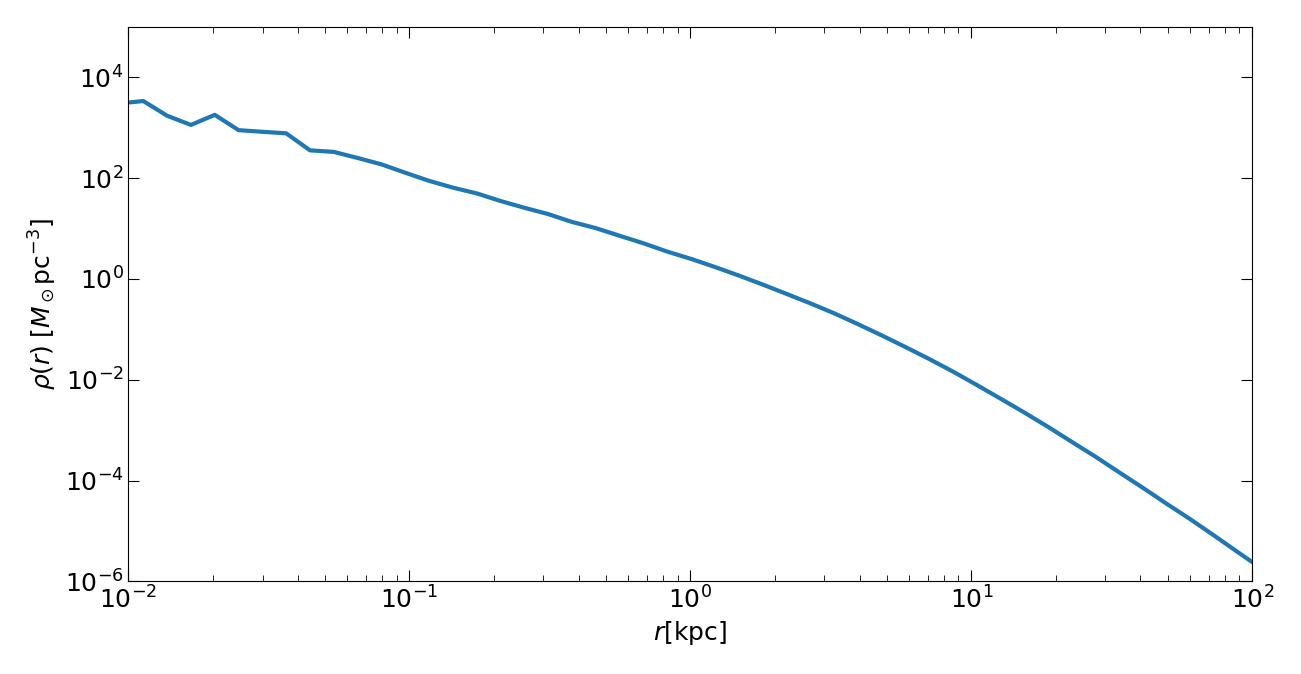
\includegraphics[width=\textwidth]{IC.png}
	\caption{Example mass density profile of the progenitor galaxies. The initial conditions for the profile in question were the same as in table \ref{table:properties}; with the exception of the number of dark matter and stellar particles, which were only $10\%$ of their respective values.}
	\label{figure:IC_density_profile}
\end{figure}

The simulations themselves thus comprise of seven mergers of two identical progenitor galaxies from table \ref{table:properties}. The galaxies are merged on a nearly parabolic orbit with an initial separation of $d = 30 \; \mathrm{kpc}$. This kind of orbit makes the approach of the galaxies swift, and causes the stellar cusps to merge before $t \sim 300 \; \mathrm{Myr}$.

The simulation data that I will be analysing, comes in the form of snapshots of the merger remnants. These snapshots are taken at the simulation time of $\sim 2 \mathrm{Gyr}$, at which point the progenitor galaxies have merged into a single merger remnant which contains an SMBH binary in its centre. The snapshots contain the positions, velocities and masses of every particle.

\section{Core Size Measurements}

In order to check if a galaxy is cored, I calculate its surface brightness profile and check if the galaxy contains regions deficient in surface brightness near its centre.

The surface brightness profiles are calculated from the merger remnant snapshots using the following procedure. First, the coordinate system is changed to centre-of-mass coordinates, after which the stellar particles are projected onto a 2D plane. Now, by calculating the mass inside logarithmically spaced radial bins, we get a radial surface mass density profile. The aforementioned calculations are repeated 100 times from random viewing angles, which results in 100 slightly different density profile projections. These profiles are then averaged azimuthally, which results in a smooth surface mass density profile, that can then be turned into a surface brightness profile by assuming a mass-to-light ratio for the stellar particles \citep{Rantala2018}. 

The simulations do not contain information about the ages and metallicities of the stellar particles, the only properties that the stellar particles have in the snapshot are: their position and velocity at a singular point in time, as well as a mass that is identical for all stellar particles. These parameters are not enough to make valid, physically accurate, assumptions on their specific mass-to-light ratios. For this reason, a constant mass-to-light ratio of $M/L = 4$ is used, which is equivalent to the ratio derived from dynamical modelling of NGC 1600 by \cite{Thomas2016}.

Figure \ref{figure:surface_brightness} shows example surface brightness profiles for every simulated merger remnant. Studying the different curves, one can already see that the presence of central SMBHs in the merger progenitors causes a clear brightness deficiency near the centre of the merger remnant. In addition, there is a systematic effect which shows that the larger the mass of the central black hole binary, the larger the amount of missing light in the core.

\begin{figure}[h]
	\centering
	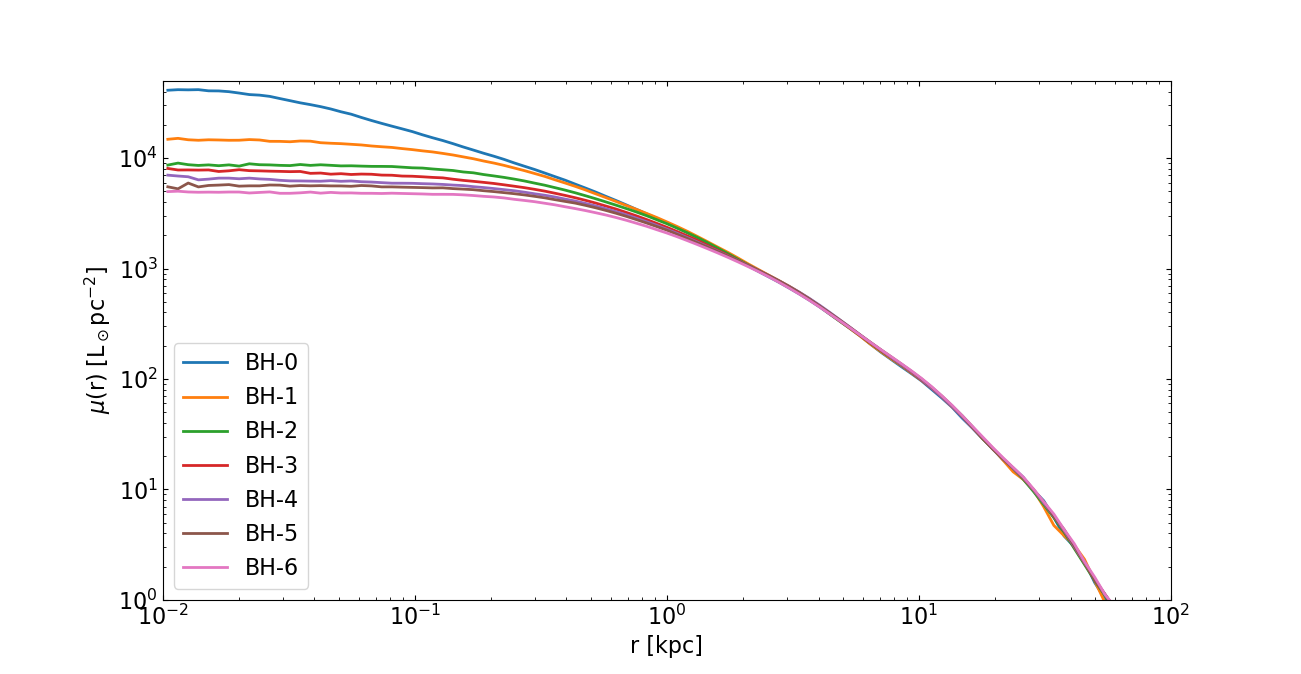
\includegraphics[width=\textwidth]{SurfaceBrightnessProfiles.png}
	\caption{Surface brightness profiles from every simulated merger remnant. These were calculated by dividing the stellar particles in the simulated galaxy remnants into 100 radial logarithmic bins, and averaging the surface brightness inside the bins through 100 random viewing angles. The luminosity of the particles was estimated by assuming a constant mass-to-light ratio of $M/L = 4$.}
	\label{figure:surface_brightness}
\end{figure}

The lack of light in the surface brightness profiles reveal the presence of cores; however, determining the precise sizes of the cores requires us to find the exact locations where the deviations from the Sérsic fit begin. This can be done by fitting the derived brightness profile with a model that is a combination of two power laws: a shallow inner power-law, and a steeper outer power-law. The radius at which the outer power-law changes into the inner power-law, i.e. the break radius $r_b$, is defined as the radius of the core. 

There are two commonly used options for modelling the surface brightness profiles. The first one is the core-Sérsic profile \citep{Graham2003}, which can be expressed using the following equation:
\begin{equation}
\mu(r) = \mu' \left[ 1 + \left( \frac{r_b}{r} \right)^\alpha \right]^{\gamma / \alpha} \exp \left\lbrace -b_n \left[ \left( r^\alpha + r_b^\alpha \right) / r_e^\alpha \right]^{1/(\alpha n)} \right\rbrace, \label{eq:core-sersic}
\end{equation}
where $r_b$ is the break radius, $\gamma$ is the logarithmic slope of the inner power-law, $\alpha$ controls the sharpness of the transition between the two power-laws, $r_e$ and $n$ are the effective half-mass radius and the Sérsic index of the outer power-law respectively, and the normalization factor $\mu'$ is defined by:
\begin{equation}
\mu' = \mu_b 2^{-\gamma/\alpha} \exp \left[ b_n \left( 2^{(1/\alpha)} r_b/r_e \right)^{1/n} \right], 
\label{eq:mu_dot}
\end{equation}
where $\mu_b$ is the surface brightness at the break radius. 

The second option is to use the so called Nuker profile \citep{Lauer1995}:
\begin{equation}
\mu(r) = 2^{(\beta - \gamma) / \alpha} \mu_b \left( \frac{r_b}{r} \right)^\gamma \left[ 1 + \left( \frac{r}{r_b} \right)^\alpha \right]^{(\gamma - \beta)/\alpha},
\label{eq:nuker}
\end{equation}
where $r_b$ is once again the break radius, $\mu_b$ is the surface brightness at the break radius, $\beta$ and $\gamma$ are the logarithmic slopes of the power-laws inside and outside of the break radius respectively, and $\alpha$ describes again the sharpness of the transition between the two slopes.

\begin{figure}[h]
	\centering
	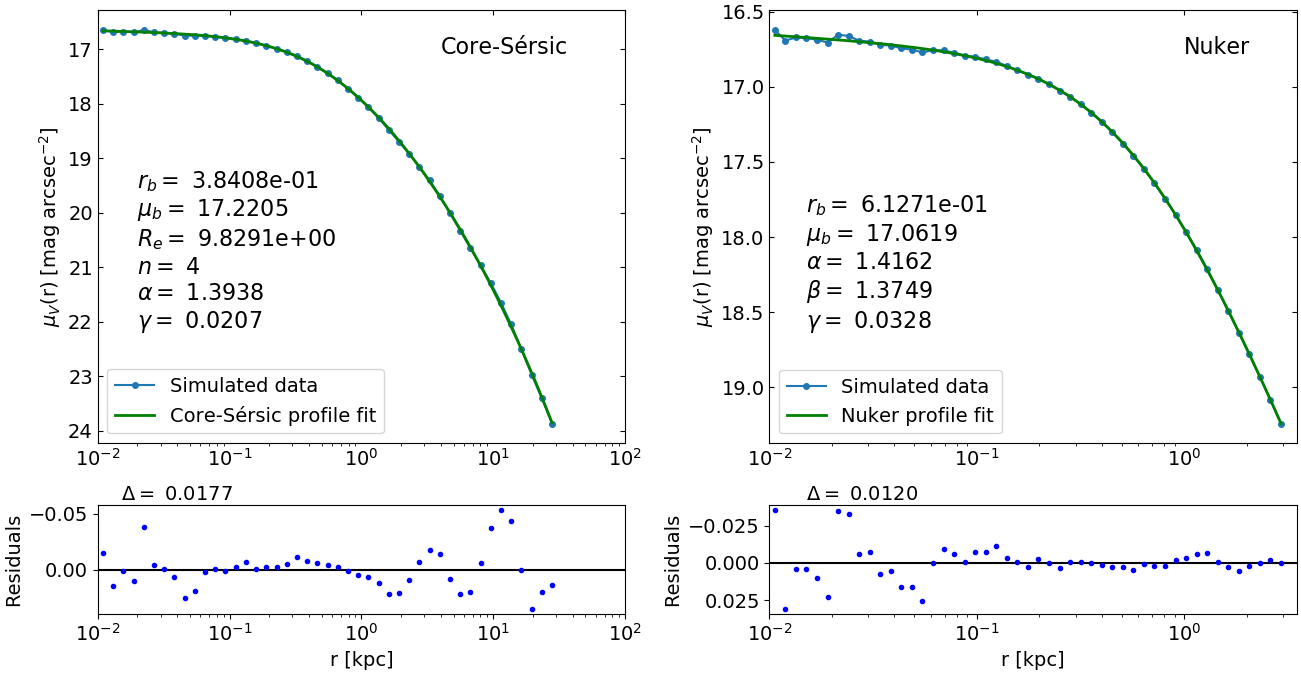
\includegraphics[width=\textwidth]{core_nuker_fits.png}
	\caption{Core-Sérsic and Nuker profile fits of surface brightness profiles calculated from the BH-3 merger remnant (left and right figures respectively). The best fit parameters are shown on the figures and are in the same units as the axes (i.e. $r_b$ and $R_e$ in kilo-parsecs, and $\mu_b$ in V-band magnitudes per arc-second squared). The relative residuals of the fits are plotted under their respective figures. The delta describes the root-mean-square of the residuals.}
	\label{figure:core_nuker}
\end{figure}

We calculate the core radii of the merger remnants by using the "Levenberg-Marquardt" fitting algorithm to fit both the core-Sérsic model and the Nuker model to the remnant's surface brightness profile. For the most part, the initial guesses of the values for the fitting parameters used in the fitting algorithm were determined through trial-and-error as well as knowledge of their likely orders of magnitude. However, while fitting the core-Sérsic profile, the Sérsic-index ($n$) was fixed to $n=4$ in order to reduce degeneracy between the fitting parameters.

Figure \ref{figure:core_nuker} shows a comparison of the resulting fits for the BH-3 merger (refer to table \ref{table:properties}), while figures \ref{figure:all_core} and \ref{figure:all_nuker} show the fits for every remnant that contains a SMBH binary. The values of the best-fit parameters are shown on the figures. The units of the surface brightness are changed from $L_\odot \; \mathrm{pc^{-2}}$ to $\mathrm{mag \; arcsec^{-2}}$ (where $\mathrm{mag}$ is the magnitude in the V-band) using the common conversion formula:
\begin{equation}
\mu = M_\odot + 21.572 - 2.5 \log(I), 
\end{equation}
where $M_\odot$ is the absolute magnitude of the Sun in a specific spectral band (in our case the V-band magnitude of $4.83$ is used), and $I$ is the surface brightness in $L_\odot \mathrm{pc^{-2}}$.

The root-mean-square of the fits' residuals are comparable to the values seen in profile fits of observed surface brightness profiles: $\Delta \approx 0.02 \; \mathrm{mag \; arcsec^{-2}}$ \citep{Dullo2012}. Although, while the RMS of the residuals show that the fits describe the surface brightness profiles rather well, most of the fits have large residual scatter near the centre of the merger remnant. This is especially noticeable in the Nuker fits, since in order to get sensible values for the fitting parameters, the fitting range needs to be concentrated in the galactic centre. However, this central residual scatter is most likely not indicative of any kind of physical merger remnant core structure; but a result of the logarithmic spacing of the bins in the surface brightness profiles. The bins near the centre are inherently smaller than the outer bins; which causes larger variation in the binned masses, and thus luminosities, when calculating the projected surface brightness profiles from different angles. This results in a final average profile, where the central regions contain small random variations in luminosity, which naturally cause the residuals of the fits to be scattered in a random way.

Interestingly, all of the core-Sérsic fits show a peak in the size of the residuals at around $\sim 10 \mathrm{kpc}$. Once again, this residual property is probably not an actual physical structure found in merger remnants. However, the fact that it appears in the surface brightness profile from every simulation indicates that; even though the masses of the SMBHs in the merger progenitors have a large effect on the central regions of the merger remnant, the outer regions are left relatively unaffected. The central SMBH binary only affects the outer regions through stellar particles that have been ejected from the galactic centre. 

All of the significant residual variations between the profile fits of the simulated merger remnant galaxies are concentrated near their respective centres. This implies that the results of the different simulations vary significantly from each other only due to the formation of a central SMBH binary, since the similar shapes of the outer regions of the residual plots can be explained through the limited range of the binaries' gravitational spheres-of-influence (SOI). The radii of the SMBH binaries' SOI can be seen in table \ref{table:s-o-i}. These were calculated by finding the radius of a sphere that contains the amount of stellar mass equivalent to the mass of the central SMBH binary in the respective galaxy, and calculating the 2D projection of the radius using the relation described in equation \ref{eq:a_star_re_relation}


\begin{table}
	\begin{center}
		\begin{tabular}{| c | c |}
		\hline
		Simulation & $r_\mathrm{SOI}$ $\mathrm{[kpc]}$ \\
		\hline
		BH-1 merger & 0.143 \\
		BH-2 merger & 0.256 \\
		BH-3 merger & 0.394 \\
		BH-4 merger & 0.515 \\
		BH-5 merger & 0.620 \\
		BH-6 merger & 0.757 \\
		\hline
		\end{tabular}
	\end{center}
	\caption{Estimations of the projected influence radii $r_\mathrm{SOI}$ for every merger remnant with a central SMBH binary. The radii are calculated by finding the radius of the sphere that contains the amount of stellar mass equivalent to the mass of the central SMBH binary, and calculating its 2D projection using the relation described in equation \ref{eq:a_star_re_relation}.}
	\label{table:s-o-i}
\end{table}

%Before studying the break radii, it is useful to also analyse some of the other fit parameters, since they might provide some interesting information about the mergers. Figure \ref{figure:all_core} shows that the central SMBH binary mass does not seem to have a systematic effect on the merger remnants' effective radii. Seeing as the central luminosity deficit grows with the binary's mass, one would assume that, in order to account for the larger amount of missing light, the effective radius would follow suit. However, as this is not the case, one may conclude that; either the larger loss in of total luminosity of the remnant already accounts for the larger luminosity deficit in the centre; or, due to some computational error, the effective radii in question do not provide physically accurate results.

%... $\alpha$ analysis? ...

\begin{figure}
	\centering
	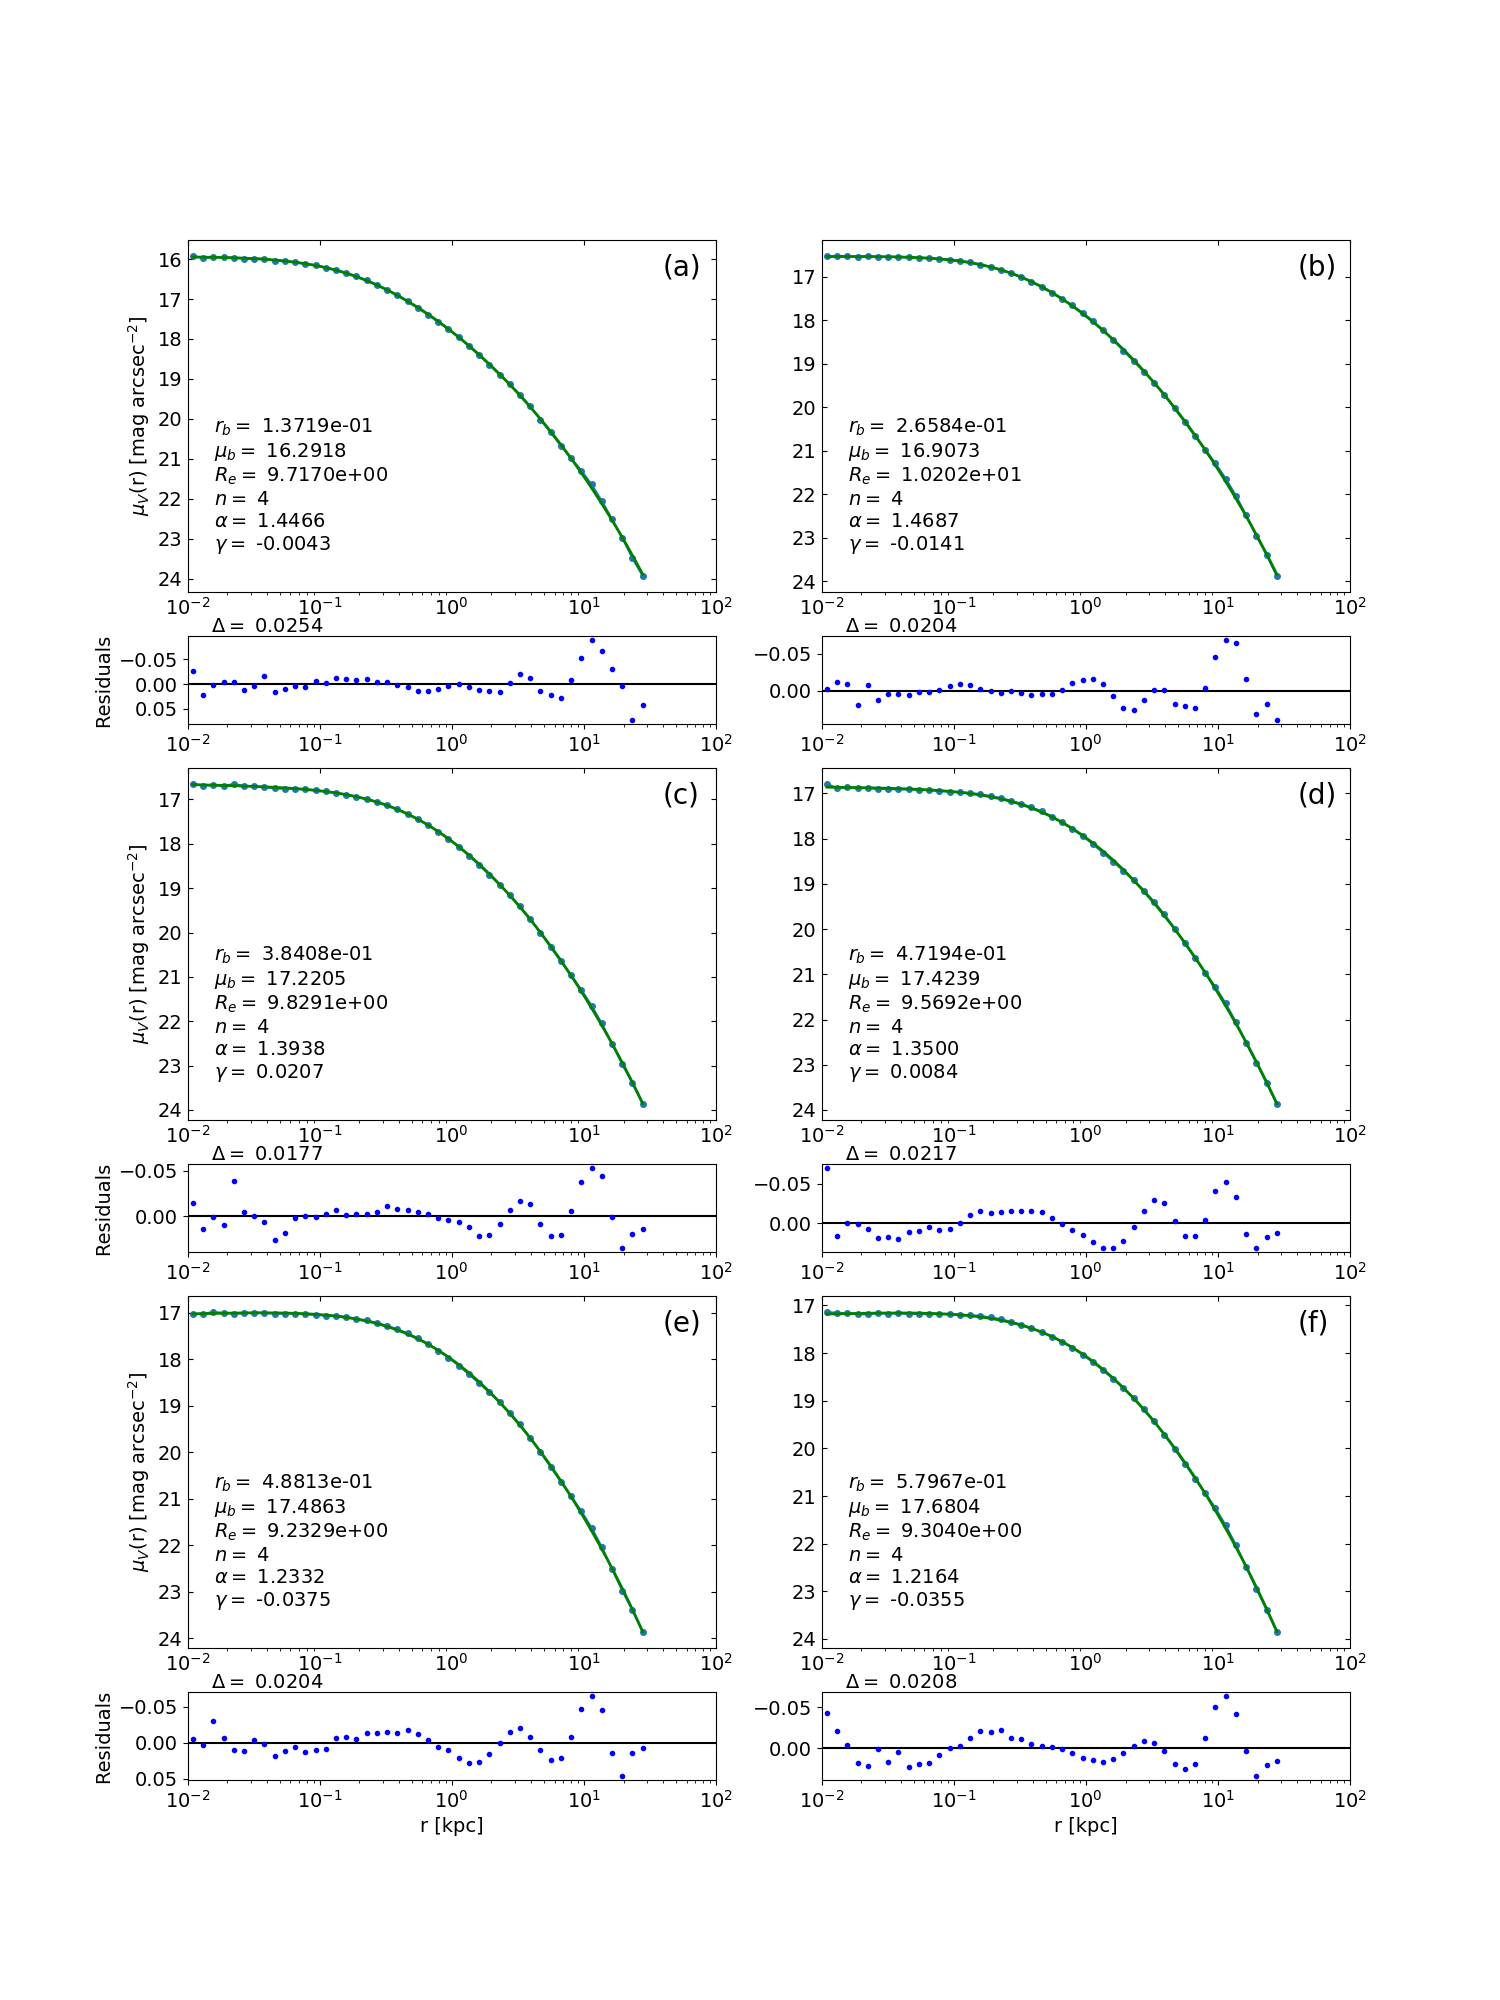
\includegraphics[width=\textwidth]{all_core_profiles.png}
	\caption{Core-Sérsic profile fits of the surface brightness data calculated from all of the individual simulated merger remnants with progenitors containing central supermassive black holes. The letters (a)-(f) denote the different snapshots ((a): BH-1 merger, (b): BH-2 merger, (c): BH-3 merger, (d): BH-4 merger, (e): BH-5 merger, (f): BH-6 merger).}
	\label{figure:all_core}
\end{figure}

\begin{figure}
	\centering
	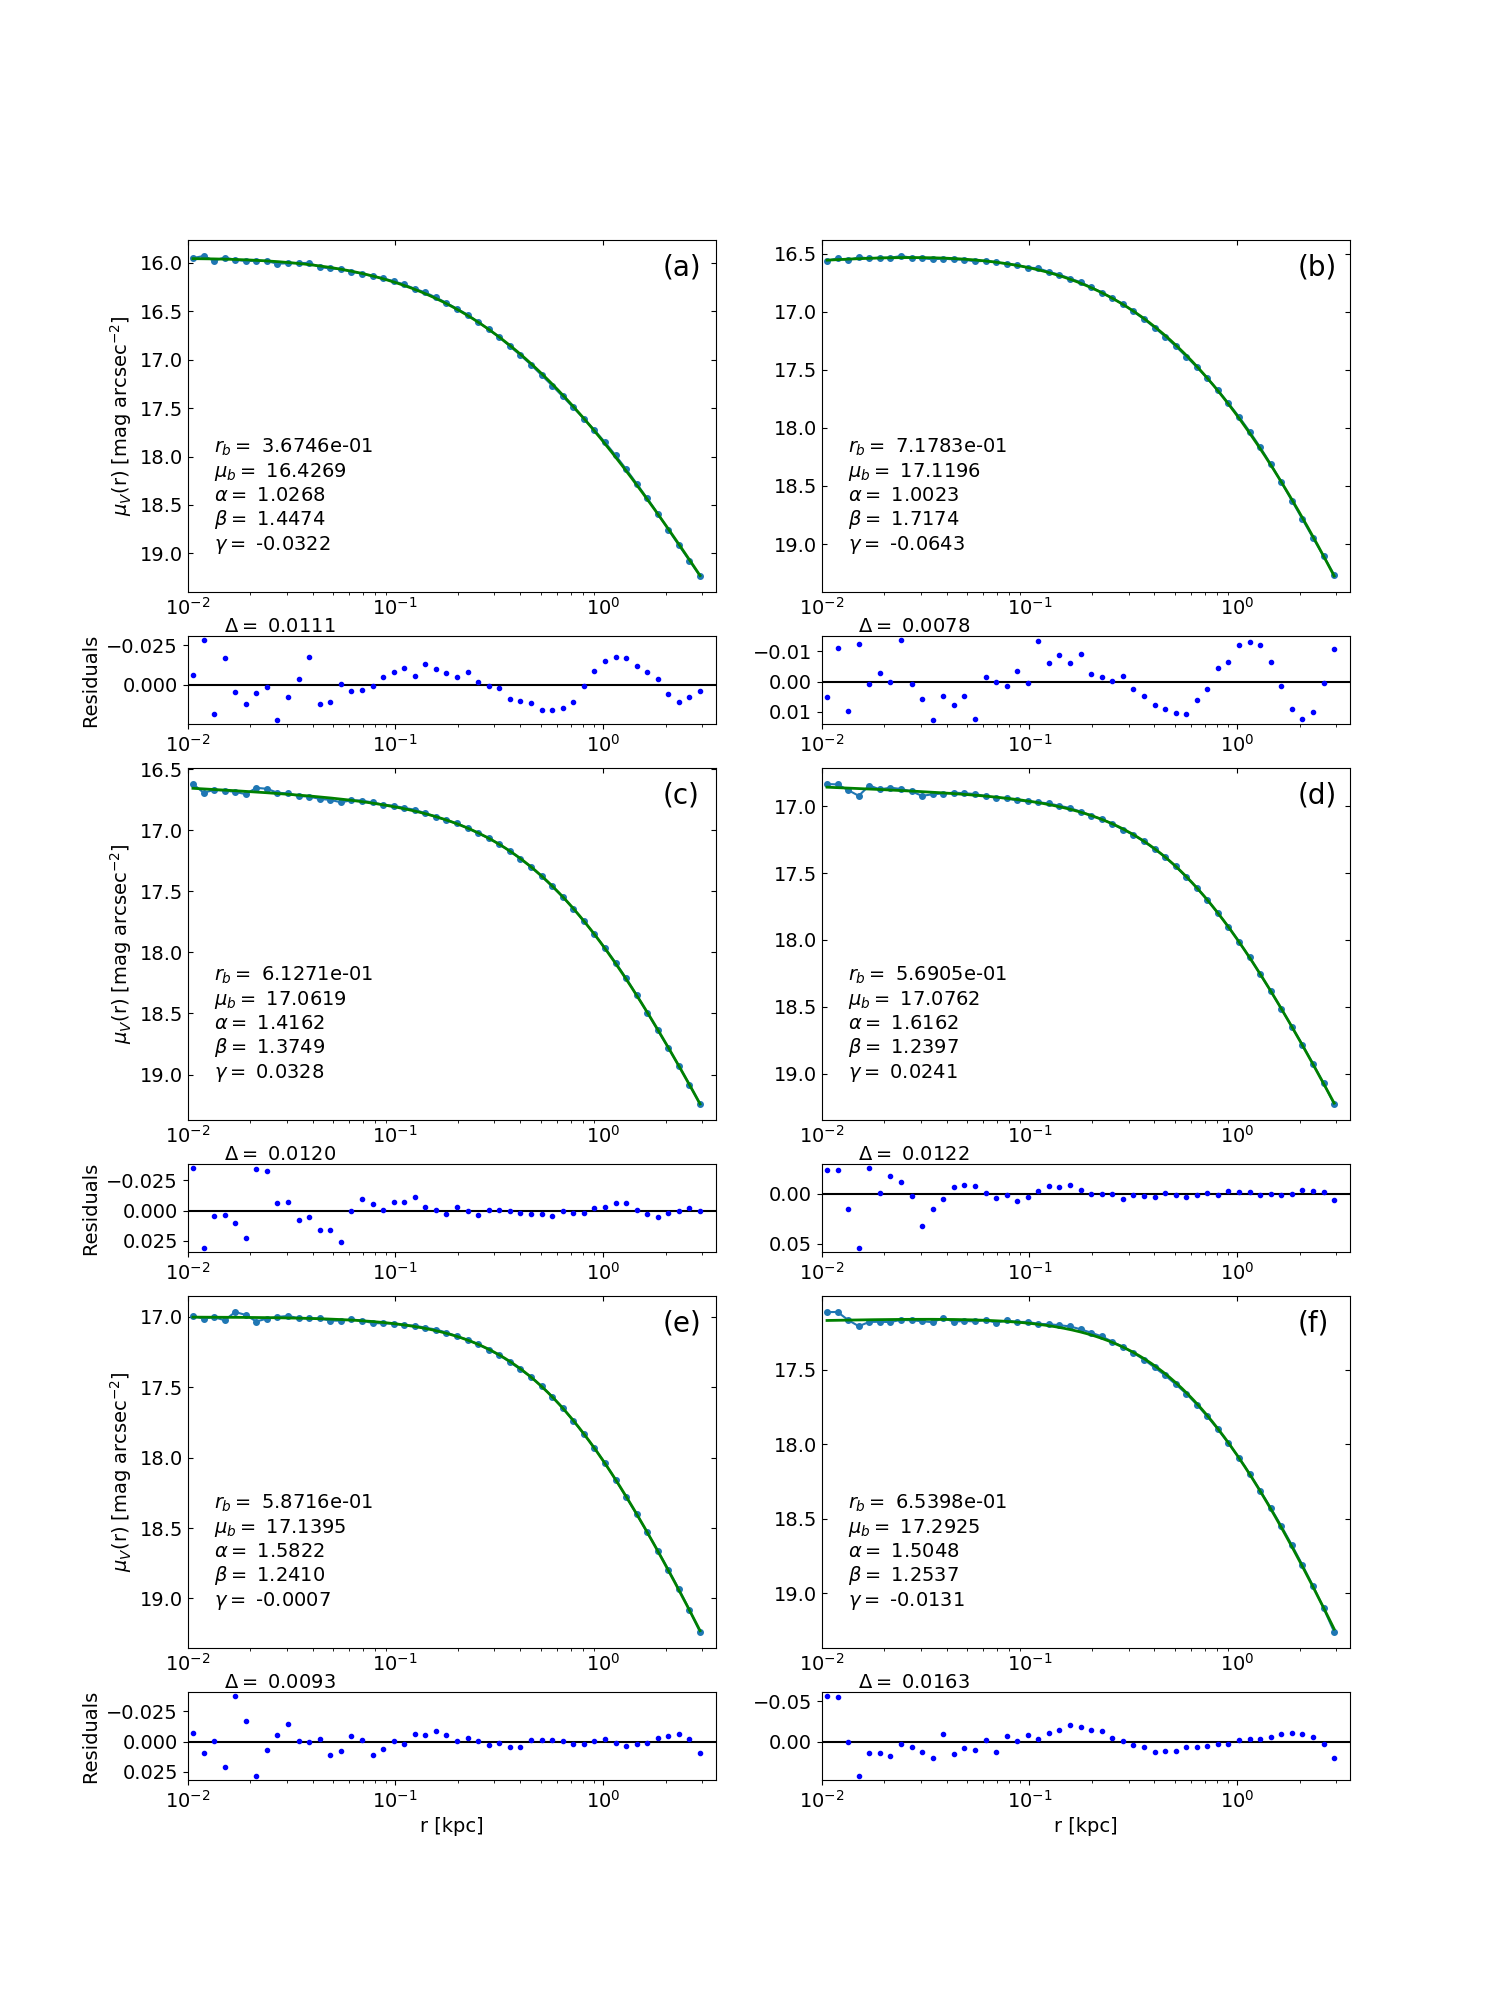
\includegraphics[width=\textwidth]{all_nuker_profiles.png}
	\caption{Nuker profile fits of the surface brightness data calculated from all of the individual simulated merger remnants with progenitors containing central supermassive black holes. The letters (a)-(f) denote the different merger remnants ((a): BH-1 merger, (b): BH-2 merger, (c): BH-3 merger, (d): BH-4 merger, (e): BH-5 merger, (f): BH-6 merger).}
	\label{figure:all_nuker}
\end{figure}

Figures \ref{figure:all_core} and \ref{figure:all_nuker} show that the core radius estimate depends quite strongly on the used fitting model. However, which model is better for estimating the size of the core is still a matter of debate \citep{Lauer2007, Dullo2012}. While the RMS of the relative residuals seems to be consistently (although just marginally) smaller for the Nuker model, when compared to the RMS for the core-Sérsic model (compare figures \ref{figure:all_core} and \ref{figure:all_nuker}), one also has to take into account that in the Nuker model the best-fit value for $r_b$ is strongly dependent on the fitting range \citep{Graham2003Nuker}. Furthermore, as stated by \cite{Rantala2018}, in order to get sensible values for all of the model parameters (e.g. $\alpha \lesssim 1$ might even prevent the model from describing the profile as a combination of two power-laws), the fitting range of the Nuker model has to be narrowed down closer to the galactic centre. This, when combined with the parameters' high dependence of the fitting range, shows that the core radius estimations of the Nuker model can be inconsistent.

In addition, one could also estimate the size of the core without model fitting by calculating the so-called "cusp radius" $r_\gamma$, i.e. the distance from the galactic centre at which the logarithmic slope of the surface brightness profile equals $\gamma' = -1/2$ \citep{Carollo1997, Lauer2007Cusp}. Because the cusp radius $r_\gamma$ also provides an estimate for the location where the inner power-law of the profile changes into the outer power-law, it can be equated to the core radius. 

We calculate $r_\gamma$ for all of the merger remnants with SMBH binaries (BH-1 - BH-6 mergers) by calculating the gradient of the surface brightness profiles, and then using a function minimization algorithm \citep{NelderMead} to minimize the difference $\big| \frac{d\mu(r)}{dr} - \left( - \frac{1}{2} \right) \big|$ in order to find the radius, at which the gradient gets the value $-1/2$. 

\begin{figure}[h]
	\centering
	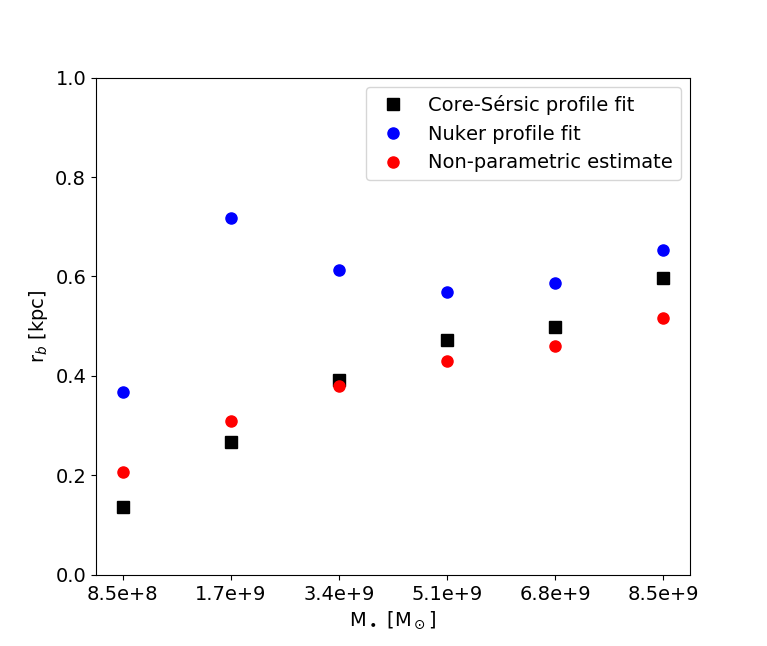
\includegraphics[width=\textwidth]{rb_mass_relation.png}
	\caption{Comparison of the core radii of the merger remnants, derived through three different methods: Core-Sérsic profile fitting (black squares), Nuker profile fitting (blue circles) and  finding the "cusp radius" (red circles). The x-axis shows the masses of the central SMBH binaries in the merger remnants.}
	\label{figure:radii_comparison}
\end{figure}

Figure \ref{figure:radii_comparison} compares the core radius estimates from each of the three methods for every simulated merger remnant. The break radii from the Nuker fits are consistently larger than the other core radius estimates. They also have, in general, the largest deviations from the other core radius estimates, and even contain two values that seem to break the trend of the core radius growing with the central SMBH binary mass (these being the break radii for the BH-2 and BH-3 mergers). Similar larger than expected Nuker core radii can be seen in the analysis of the simulations by \cite{Rantala2018}. Much like in figure \ref{figure:radii_comparison}, the difference in their Nuker break radii and the other core radius estimates for the two mergers with the smallest and third smallest central SMBH binaries, are significantly larger than for the other mergers. The fact that these large deviations are present in both our analysis and the analysis by \cite{Rantala2018}, further implies that, due to its high dependence on the fitting range, the Nuker model can provide inconsistent values for the break radius. When excluding these few Nuker break radii, a clear trend of the size of the core growing with the merger progenitors' central SMBH masses can be seen.

The fact that the size of the core is dependent on the mass of the central SMBH binary is clear evidence towards the cores being formed through a scouring process by the binary black holes. Binaries with larger masses have larger gravitational spheres-of-influence (table \ref{table:s-o-i}), which naturally leads to the ejection of stellar particles that orbit farther away from the galactic centre (the larger SMBH binary mass also causes the stellar material to be ejected at a larger velocity). 

This positive correlation between the core size and the SMBH binary mass has also been identified in independent measurements of the break radius and the central SMBH mass in cored galaxies \citep[e.g.][]{deRuiter2005, Lauer2007Cusp, Thomas2016}. The fact that this effect can be seen, not only in the simulations but also in the observations, makes it clear that merging SMBH binaries are a likely source for the core.

Alongside the size of the core, the surface brightness deficit also becomes larger as the central SMBH binary mass grows, as can clearly be seen in figure \ref{figure:surface_brightness}. This can be explained trough the concept of the loss-cone. \cite{BinneyTremaine} show that only stars with the angular momentum:
\begin{equation}
L \lesssim [G(M_1 + M_2)a]^{1/2}, \label{eq:loss-cone}
\end{equation}
where $M_1$ and $M_2$ are the masses of the binary black holes, interact strongly enough with the binary to be ejected from the system (i.e. are inside the loss-cone). As the above equation implies, the upper limit of this condition grows alongside the binary mass. This causes more of the orbiting stellar particles to be located in the strong interaction range; as not only does the loss-cone widen, allowing for the ejection of particles with orbits more parallel to the plane of the binary; but the maximum velocities, at which a stellar particle can interact strongly with the binary, also become larger. Thus, a larger SMBH binary mass naturally results in the ejection of a larger number of stellar particles, which then leads to the growth of the central surface brightness deficit.  

\section{Velocity Anisotropy}

%\begin{figure}[h]
%	\centering
%	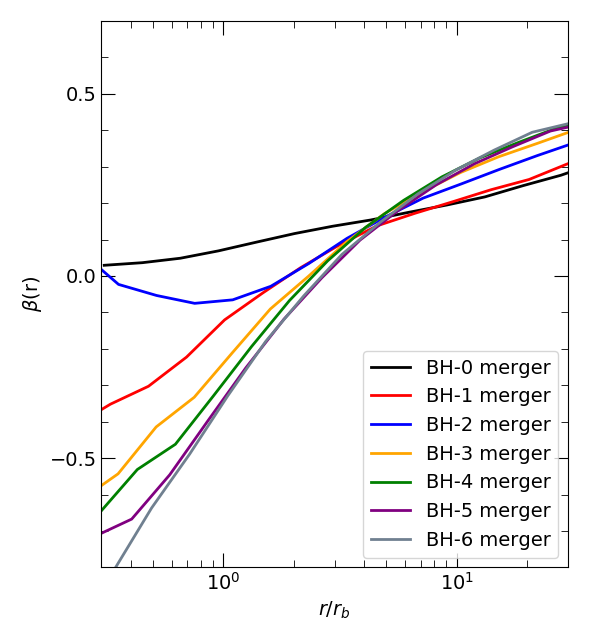
\includegraphics[width=0.9\textwidth]{beta.png}
%	\caption{Velocity anisotropy (beta) profiles of the simulated merger remnants with central black holes.}
%\end{figure}

Another method of studying whether a galaxy has formed a core through core scouring by binary black holes, is to study the velocity anisotropy profile defined in \cite{BinneyTremaine} as:
\begin{equation}
\beta(r) = 1 - \frac{\sigma_\theta^2 + \sigma_\phi^2}{2\sigma_r^2} = 1 - \frac{\sigma_t^2}{\sigma_r^2}, \label{eq:beta}
\end{equation}
where $\sigma_\theta$, $\sigma_\phi$ and $\sigma_r$ are one dimensional velocity dispersions in the spherical coordinates, and $\sigma_t = \sqrt{(\sigma_\theta^2 + \sigma_\phi^2) / 2}$ is the tangential velocity dispersion. This $\beta$-parameter describes the ratio of tangential velocity dispersion in the stellar system to the radial velocity dispersion and, as such, provides information about the nature of the stellar orbits around the black hole binary. A negative value for $\beta$ shows an abundance of tangential orbits, where as a positive $\beta$ corresponds to an abundance of radial orbits. 

Figure \ref{figure:beta_no_rb} shows $\beta$-profiles calculated from all of the final merger remnant snapshots using equation \ref{eq:beta}. In order to get the velocity dispersions, the stellar particles of the remnant were first divided into logarithmic bins, and their velocities were changed from a Cartesian to a spherical coordinate system. Next, the root-mean-squares, which correspond to the velocity dispersions, of the different spherical velocity components were calculated for each bin separately, resulting in a $\beta$-value for every bin. Plotting these values gives us the aforementioned profiles in figure \ref{figure:beta_no_rb}. 

\begin{figure}[h]
	\centering
	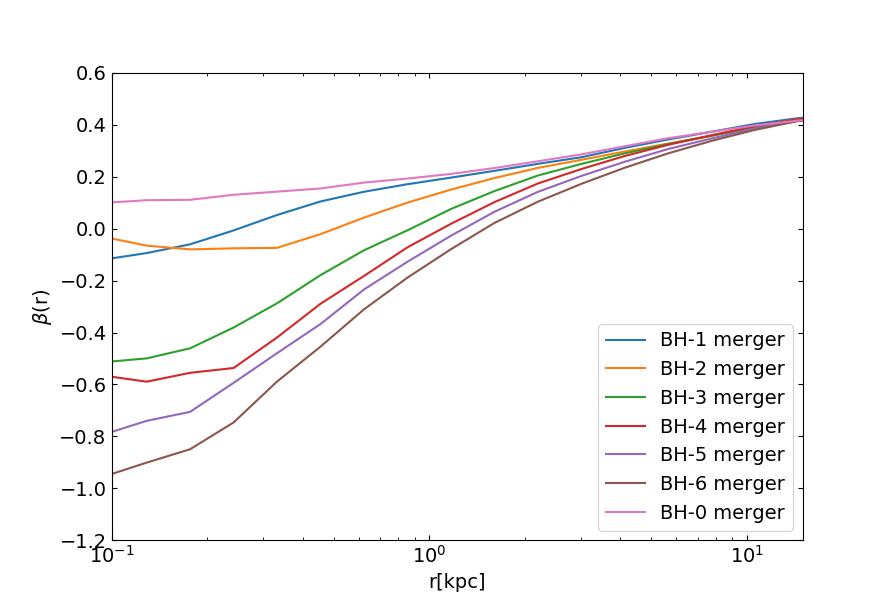
\includegraphics[width=0.9\textwidth]{beta_no_rb.png}
	\caption{Velocity anisotropy (beta) profiles for every simulated merger remnant. The profiles are calculated from the velocity dispersions in radial logarithmic bins, using equation \ref{eq:beta}. As the profile goes from the outer regions of the merger remnants to the central regions, the profiles of the remnants with SMBH binaries go from being radially dominated to tangentially dominated.}
	\label{figure:beta_no_rb}
\end{figure}

According to the $\beta$-profiles, the outer areas of the remnants are dominated by radial orbits (positive $\beta$), while the majority of orbits near the centre are tangential (negative $\beta$). As the initial merger progenitors used in the simulations contained isotropic $\beta$-profiles ($\beta = 0$), an area with negative $\beta$ in the merger remnant would imply that the stars on radial orbits have been lost from the system. It has been shown that hardening black hole binaries can eject stars on highly radial orbits from the galactic core, which results in the central region becoming dominated by mostly tangential orbits (and thus a negative $\beta$). The ejected stars can, in turn, cause the outer orbits to become more radial \citep{Quinlan1997, Milosavljevic2001, Thomas2014}. 

The figure clearly shows that the presence of an SMBH binary has an effect on the profiles' shape; as not only does the slope of the profile steepen as the mass of the SMBH binary grows; but the only merger with a profile, completely dominated by the radial velocity dispersion, is the one without a central binary (the BH-0 merger). 

The profiles also make sense in the context of ejection of stellar particles by hardening black hole binaries. The larger the mass of the SMBH biary is, the larger its gravitational sphere-of-influence, which results in more of the radially orbiting stellar particles being ejected.

\begin{figure}
	\centering
	\begin{subfigure}[b]{0.39\textwidth}
		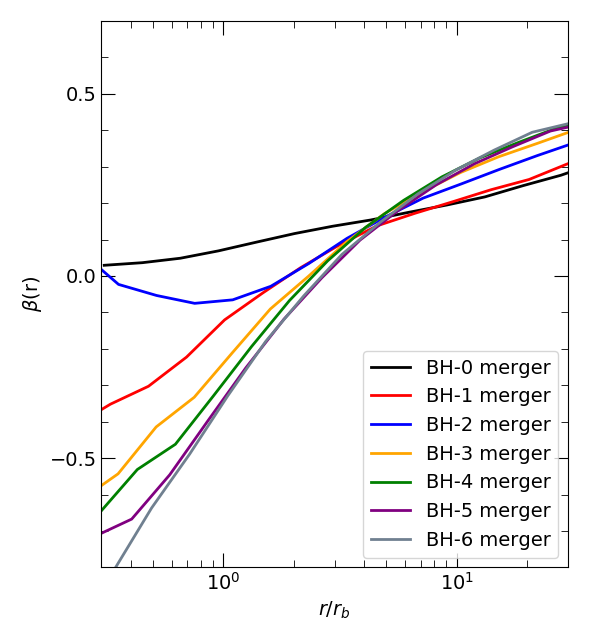
\includegraphics[width=\textwidth]{beta.png}	
		\caption{Simulated merger remnants}
	\end{subfigure}
	\begin{subfigure}[b]{0.60\textwidth}
		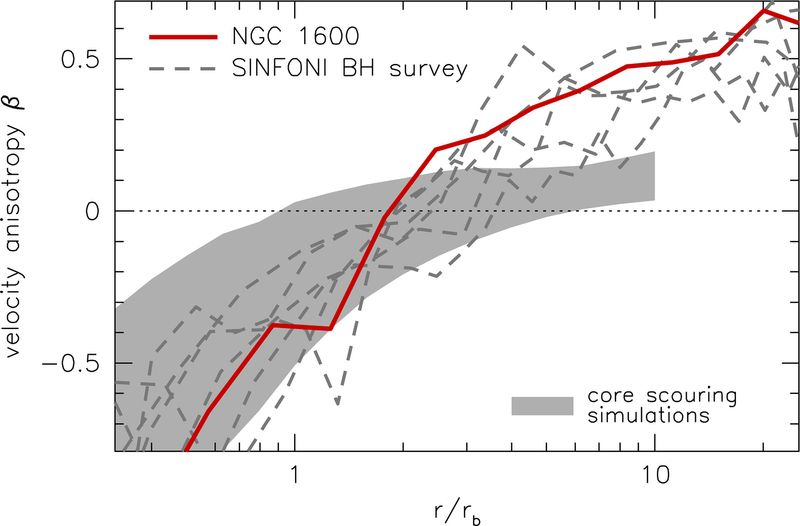
\includegraphics[width=\textwidth]{thomas2016.jpg}
		\caption{NGC 1600}
	\end{subfigure}
	\caption{(a): $\beta$-profiles of the simulated merger remnants as a function of distance from the centre scaled by their respective break radius. For the merger remnant without a core (BH-0), the value used for the break radius is $r_b = 1 \; \mathrm{kpc}$. The profile for the BH-2 merger shows an increase in the value of $\beta$ near the centre of the merger remnant, which is simply the same increase seen in figure \ref{figure:beta_no_rb} but amplified by the break radius scaling. (b): $\beta$-profile of NGC 1600, alongside profiles of galaxies from the SINFONI black hole survey (references), and the range of anisotropies found in N-body simulations of the core scouring mechanism \citep{Thomas2016}.}
	\label{figure:beta_NGC1600_Simul}
\end{figure}

Figure \ref{figure:beta_NGC1600_Simul} shows, both the observed $\beta$-profile for NGC 1600 and the profiles from the simulated merger remnants, scaled by the core radius of the respective galaxy. Even by eye, it can clearly be seen that the $\beta$-profiles from both the simulations and the observations of NGC 1600 are similar to each other (not counting the anomalous profile for the BH-2 merger). However, looking closely at the values on the axes of the plots, the observed profile of NGC 1600 seems to be  somewhat steeper than any of the simulated ones.

%According to \cite{Rantala2018} it is likely that, the larger steepness of the profile seen in NGC 1600 is due the simulations only comprising a single generation of completely isotropic ($\beta = 0$) mergers. Most observed cored galaxies, including NGC 1600, are most likely the result of multiple generations of mergers. The progenitors of the observed major merger remnant galaxy would thus have already had tangentially biased $\beta$-profiles, leading to a remnant with an even steeper profile.

According to \cite{Rantala2018}, the kinematics being more tangential close to the core in NGC 1600 than in the simulations, could be caused by further adiabatic growth of the merged central SMBH's mass. \cite{Young1980} shows that black holes that grow adiabatically through, for example accretion of gas, can cause the surrounding stellar orbits to become more tangential. If the time scale of the mass growth is smaller than the relaxation time scale of the galaxy while also being larger than the dynamical time scale of the stellar system, the growth can be considered adiabatic. This results in the conservation of the angular momentum and the radial action of the stellar orbits (radial action being one of the momenta in the canonical Hamiltonian coordinates called \textit{angle-action variables} \citep{BinneyTremaine}), which, due to the now higher gravitational potential induced by the central black hole, causes the orbits to become more circular. Although this effect is not strong enough to account for the entire shape of the $\beta$-profile, it could certainly be a reason for the more tangentially dominated core regions seen in the observations.

As for the outer region of the $\beta$-profile of NGC 1600, it is possible, that the reason why it is more radially dominated than any of the outer parts in the simulated merger remnants, is due to the lack of minor-mergers in the simulations \citep{Rantala2018}. These minor-mergers would deposit all of their mass in the outer regions of the galaxy, and would thus only disrupt the outer stellar orbits, making some of the tangential orbits more radial. Furthermore, they would not contribute to the destruction of radial orbits near the centre of the galaxy, as the smaller progenitor galaxy would not contain a central SMBH.

\section{Line-of-Sight Kinematics}

\subsection{2D Kinematic Maps}

In order to make sure that the KETJU simulations produce results which are in agreement with observations, I  also analyse the line-of-sight (LOS) kinematics of the simulated merger remnants. The analysis is focused on four different LOS velocity distribution parameters: the average LOS velocity $V_\mathrm{avg}$, the velocity dispersion $\sigma$, and the $h_3$ and $h_4$ parameters which correspond to the skewness and the kurtosis of the distribution respectively. The distribution from which these properties are calculated is defined as the following modified Gaussian function \citep{VanDerMarel1993, Bender1994}:
\begin{equation}
f(v) = I_0 e^{-\gamma^2/2}(1 + h_3 H_3(y) + h_4 H_4(y)), \label{eq:mod_gaussian}
\end{equation} 
where $I_0$ is a normalization constant, $\gamma$ is the central slope of the particle density profile, $y = (v - V_\mathrm{avg})/\sigma$, and $H_3$ and $H_4$ are the third and fourth order Hermite polynomials respectively:
\begin{eqnarray}
H_3(y) = \left(2\sqrt{2}y^3 - 3\sqrt{2}y\right) / \sqrt{6}, \\
H_4(y) = \left(4y^4 - 12y^2 + 3 \right) / \sqrt{24}.
\end{eqnarray}

The above properties are calculated using a Python-script (Matteo Frigo, internal communication), which makes use of the Voronoi tessellation algorithm by \citep{Cappellari2003} in order to provide binned statistics of the LOS velocities. First, when using the script, the "line-of-sight" is defined as the intermediate axis of the merger remnant, after which the remnant is oriented accordingly using the inertia tensor. The 2D line-of-sight projection of the remnant is then divided into "spaxels" (or simply bins) using the aforementioned Voronoi tessellation algorithm. The shape and size of the spaxels are determined so that each one contains the same signal-to-noise ratio, which in our simulated case is defined as the number of stellar particles. The LOS-velocities inside the spaxels are then made into a histogram, into which the modified Gaussian function described in equation \ref{eq:mod_gaussian} is fitted. This gives the values of the LOS-velocity distribution parameters: $V_\mathrm{avg}$, $\sigma$, $h_3$ and $h_4$ for the spaxel in question. Finally, the values of the spaxels can be plotted, resulting in 2D voronoi binned maps of all of the four parameters.

Figure \ref{figure:IFU-maps} shows the voronoi binned 2D maps of the four LOS velocity distribution parameters for the simulated BH-0 merger (no central SMBH) and the BH-6 merger (largest central SMBH), as well as for two observed galaxies NGC 3414 and NGC 4111. The contours, which are added to help visualise the shape of the galaxy, denote flux isophotes of the merger remnants, and have a spacing of one magnitude. Similar maps for the rest of the simulated merger remnants can be seen in figure \ref{figure:rest_of_voronoi}.

The IFU maps in figures \ref{figure:IFU-maps} and \ref{figure:rest_of_voronoi} show that the average LOS velocities of the simulated merger remnants are far from isotropic, with most of the remnants containing central binary SMBHs showcasing counter-rotating central regions also known as "kinematically decoupled cores" (KDC). Some of the simulated remnants (BH-4 - BH-6 mergers) even contain another counter rotating structure inside the KDC \citep{Rantala2019}. These features, alongside the relatively low average LOS-velocities, are often found in galaxies called "slow rotators" \citep{Emsellem2007}. Slow rotator galaxies are early-type galaxies which are assumed to have been formed through gas-poor "dry" mergers \citep{Emsellem2007, Cappellari2007}; processes not unlike the ones simulated in our simulations. As such, the merger remnants being slow rotators is a somewhat expected result.

\begin{figure}
	\centering
	\begin{subfigure}[b]{0.49\textwidth}
		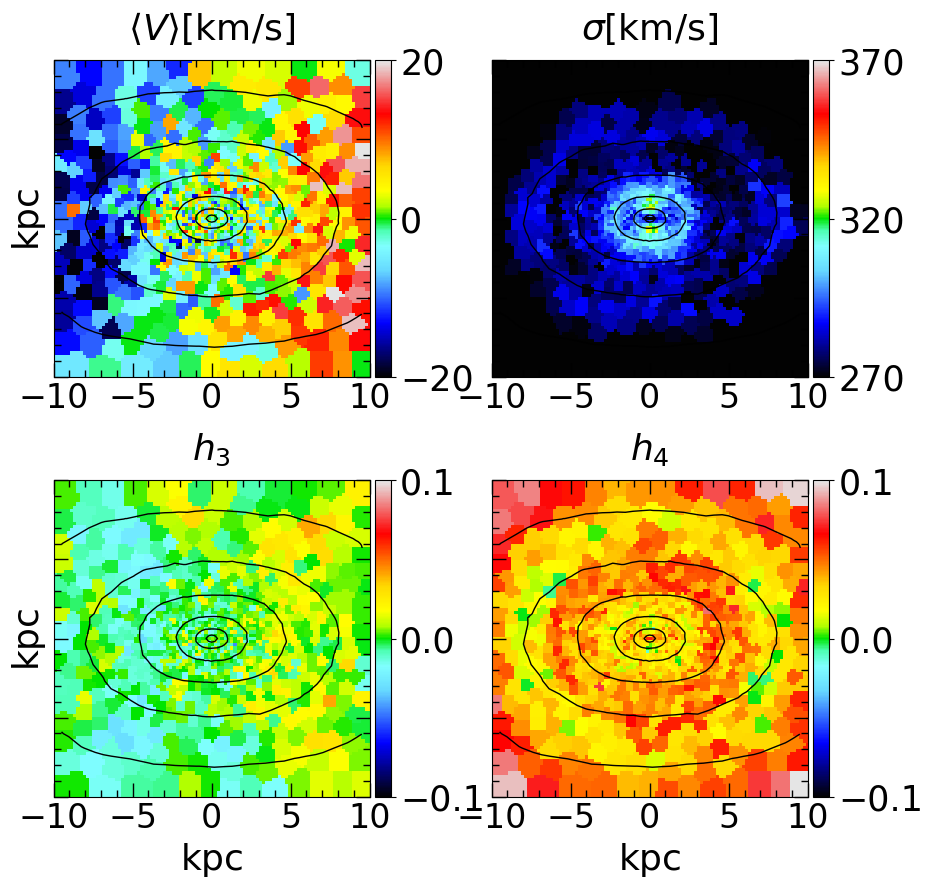
\includegraphics[width=\textwidth]{BH_0.png}
		\caption{BH-0 merger remnant}
	\end{subfigure}
	\begin{subfigure}[b]{0.49\textwidth}
		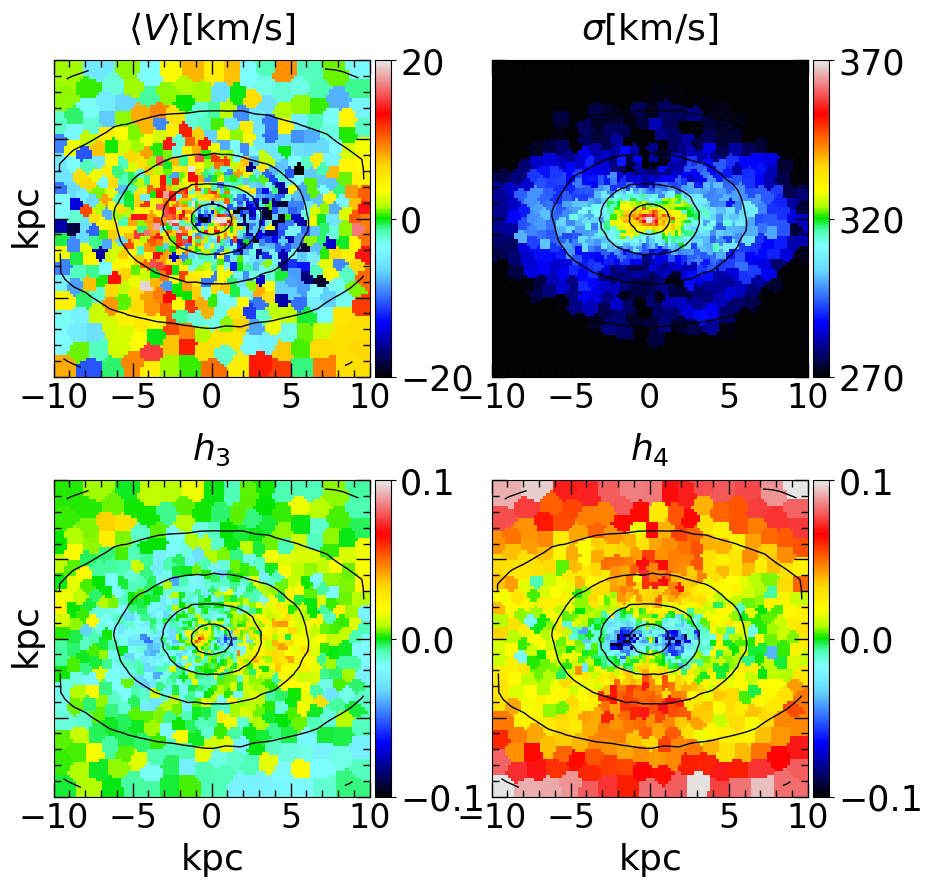
\includegraphics[width=\textwidth]{BH_6.png}
		\caption{BH-6 merger remnant}
	\end{subfigure}
	\begin{subfigure}[b]{0.49\textwidth}
		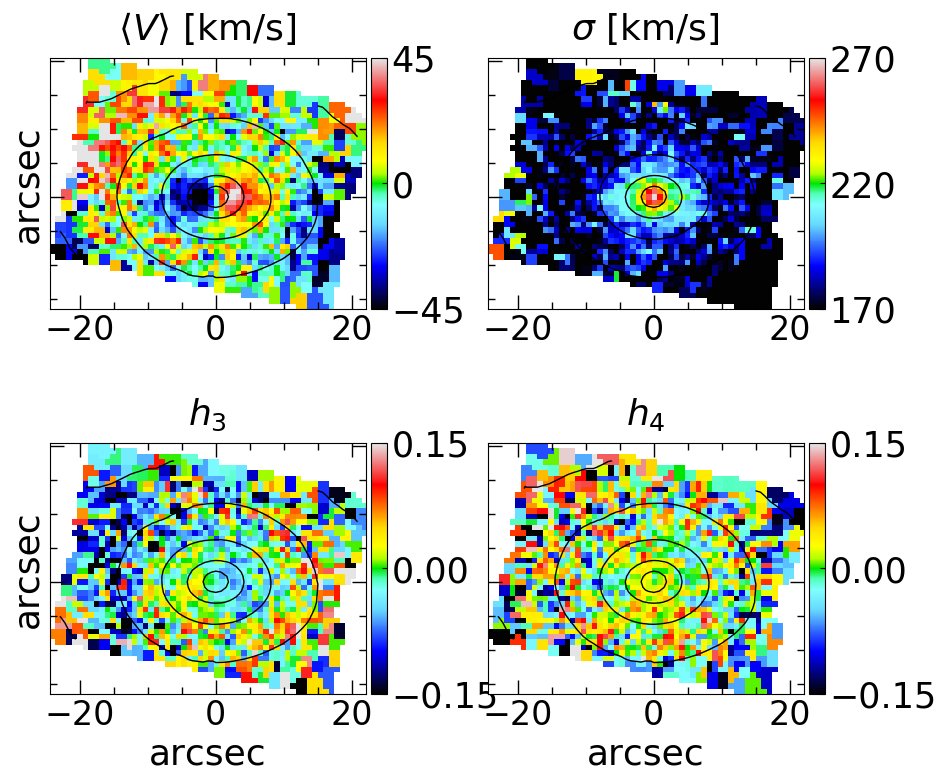
\includegraphics[width=\textwidth]{NGC3414_r6_voronoi.png}
		\caption{NGC 3414}
	\end{subfigure}
	\begin{subfigure}[b]{0.49\textwidth}
		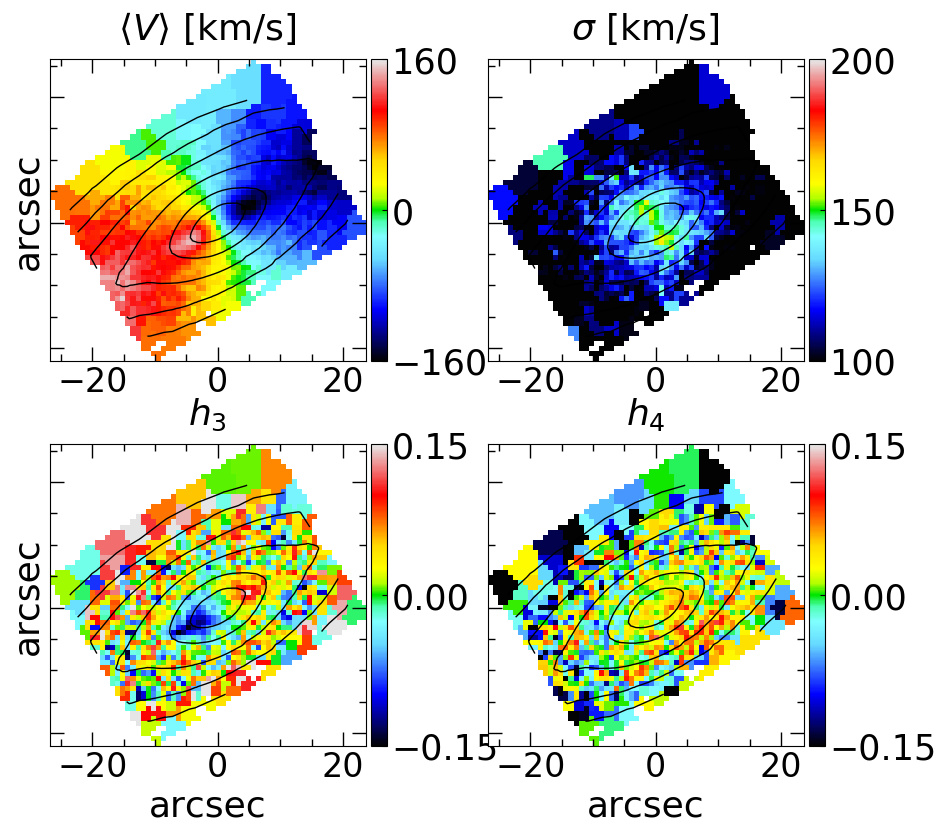
\includegraphics[width=\textwidth]{NGC4111_r1_voronoi.png}
		\caption{NGC 4111}
	\end{subfigure}
	\caption{IFU-maps of average LOS-velocities, velocity dispersion, $h_3$ parameters and $h_4$ parameters from two simulated merger remnants and two observed galaxies. The four maps in figure (a) are from the BH-0 merger, and the four in figure (b) are the BH-6 merger. Figures (c) and (d) show IFU-maps of known slow (NGC 3414) and fast rotator (NGC 4111) galaxies from the $\mathrm{ATLAS^{3D}}$ survey \citep{Emsellem2004, Cappellari2011, Krajnovic2011}.}
	\label{figure:IFU-maps}
\end{figure}

Figures \ref{figure:IFU-maps} and \ref{figure:rest_of_voronoi} also contain IFU-maps of the velocity dispersion in the simulated merger remnants. These maps show a clear connection between the mass of the central SMBH binary and the velocity dispersion at the centre of the galaxy. The presence of an SMBH binary causes the formation of a central velocity dispersion peak in the $\sigma$-distribution, the strength of which correlates positively with the mass of the binary. Furthermore, as the mass of the SMBH binary grows, the size of the area with the highest velocity dispersion in the galaxy also grows. Additionally, the growing binary mass seems to cause the high-$\sigma$ area to get more and more aligned with the major-axis of the galaxy. All of these effects can easily be identified when comparing the IFU-maps of the different simulated merger remnants from figure \ref{figure:rest_of_voronoi}, while the formation of the velocity dispersion peak caused by the simple presence of the SMBH binary is demonstrated in the IFU-maps of the BH-0 and BH-6 merger remnants in figure \ref{figure:IFU-maps}. The positive correlation between the mass of the central SMBH (or in the case of the simulations: central SMBH binary) and the velocity dispersion of its host galaxy has been observed in a multitude of galaxies with central SMBHs, both cored and non-cored \citep{Ferrarese2000}.

\begin{figure}
	\centering
	\begin{subfigure}[b]{0.49\textwidth}
		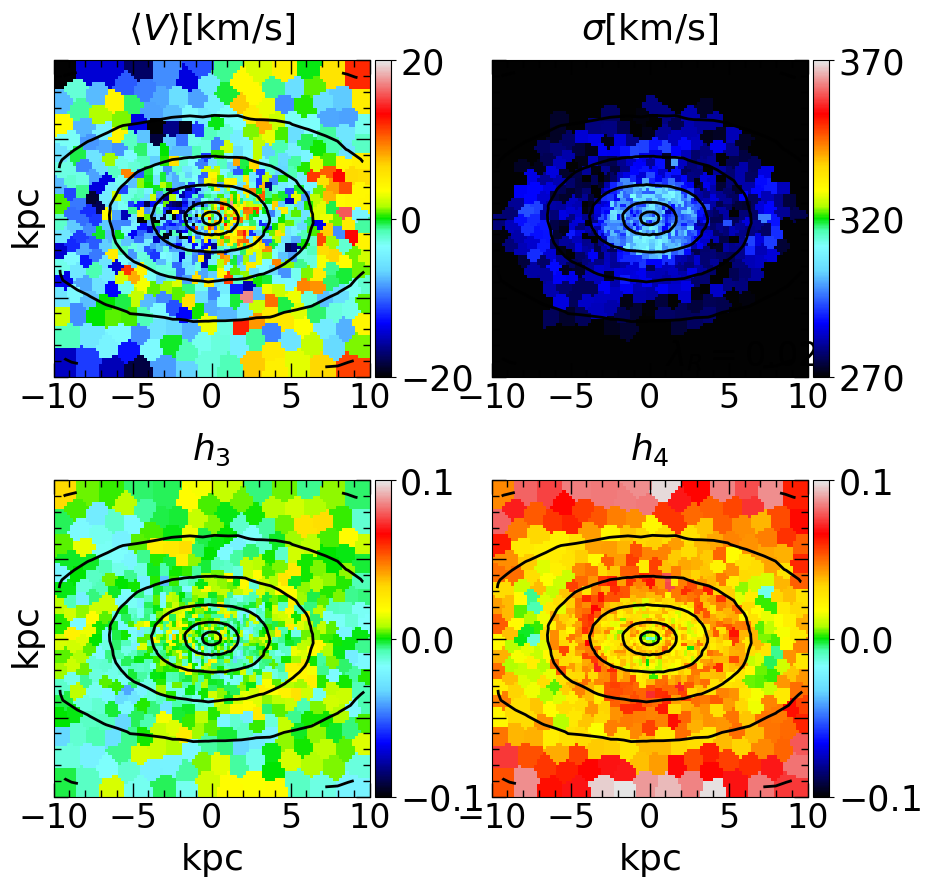
\includegraphics[width=\textwidth]{BH_1.png}
		\caption{BH-0 merger}
	\end{subfigure}
	\begin{subfigure}[b]{0.49\textwidth}
		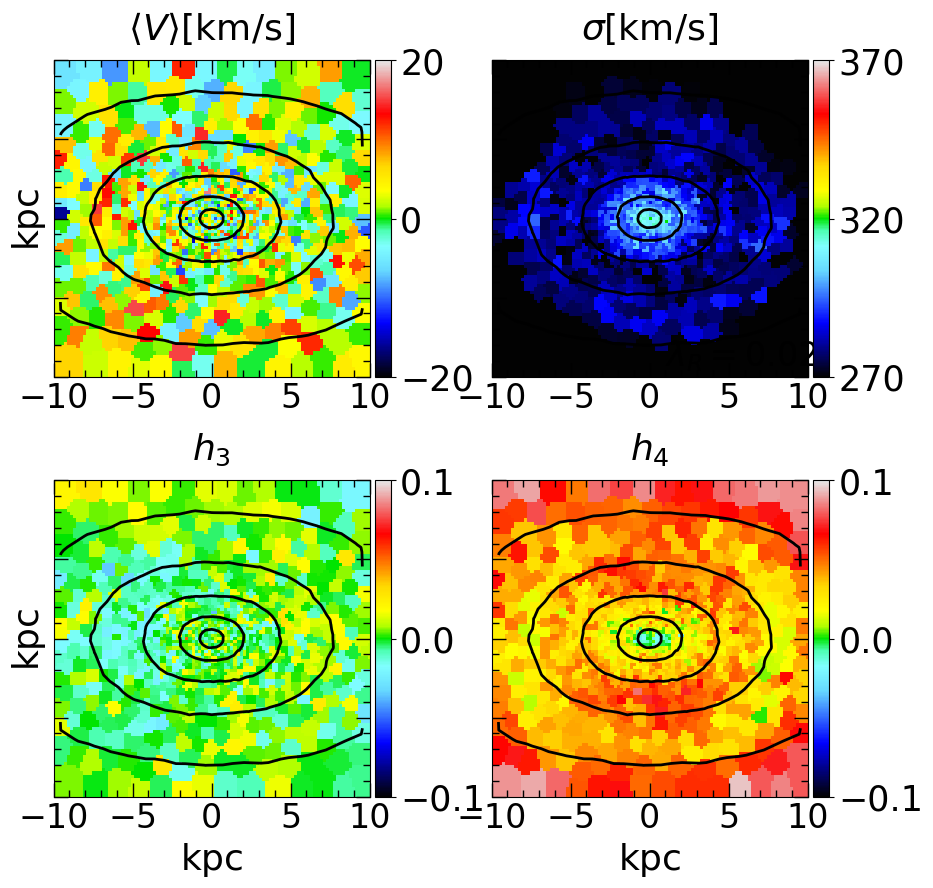
\includegraphics[width=\textwidth]{BH_2.png}
		\caption{BH-1 merger}
	\end{subfigure}
	\begin{subfigure}[b]{0.49\textwidth}
		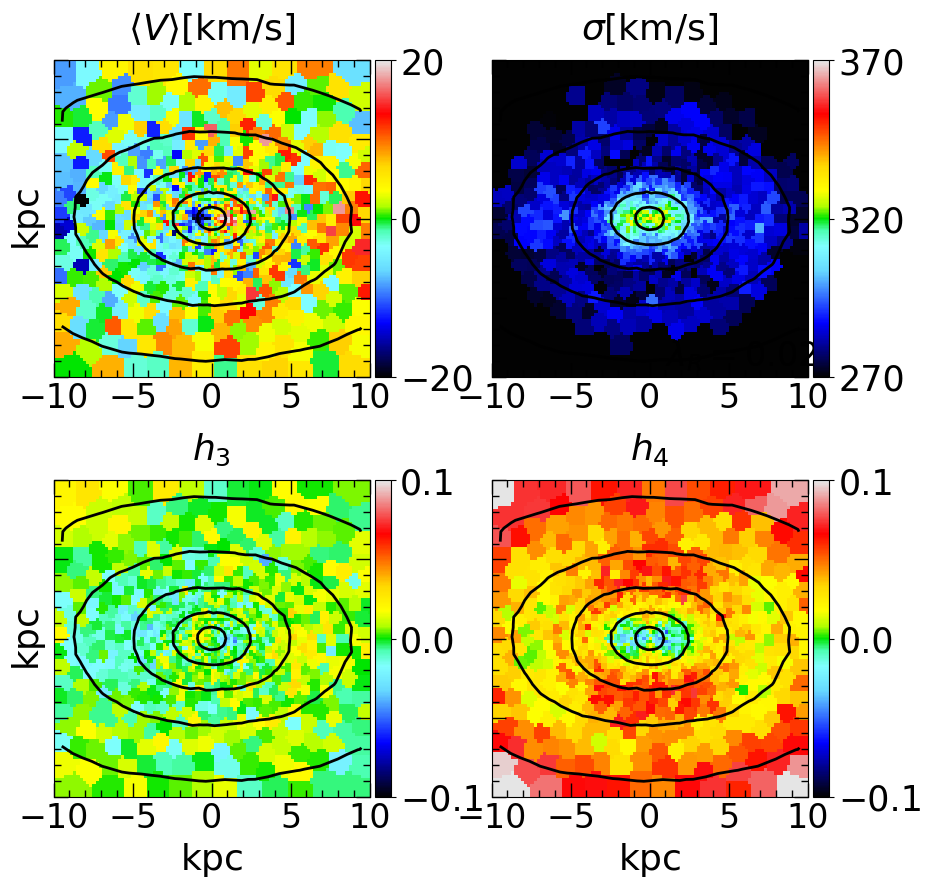
\includegraphics[width=\textwidth]{BH_3.png}
		\caption{BH-2 merger}
	\end{subfigure}
	\begin{subfigure}[b]{0.49\textwidth}
		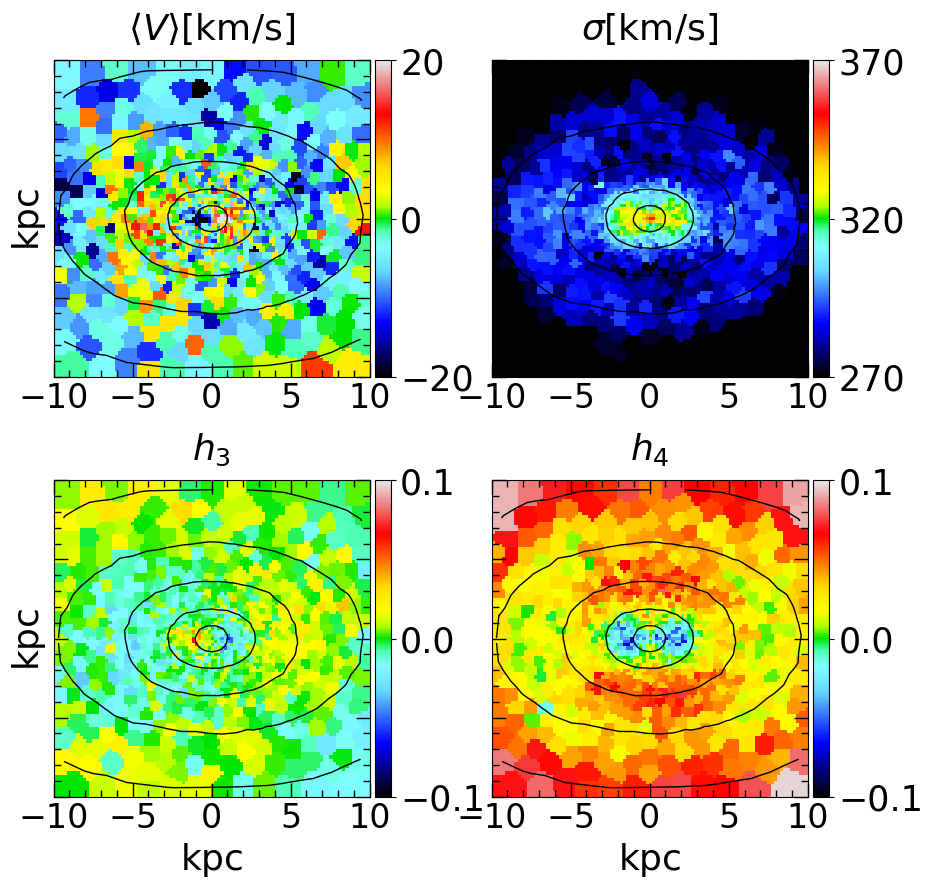
\includegraphics[width=\textwidth]{BH_4.png}
		\caption{BH-3 merger}
	\end{subfigure}
	\begin{subfigure}[b]{0.49\textwidth}
		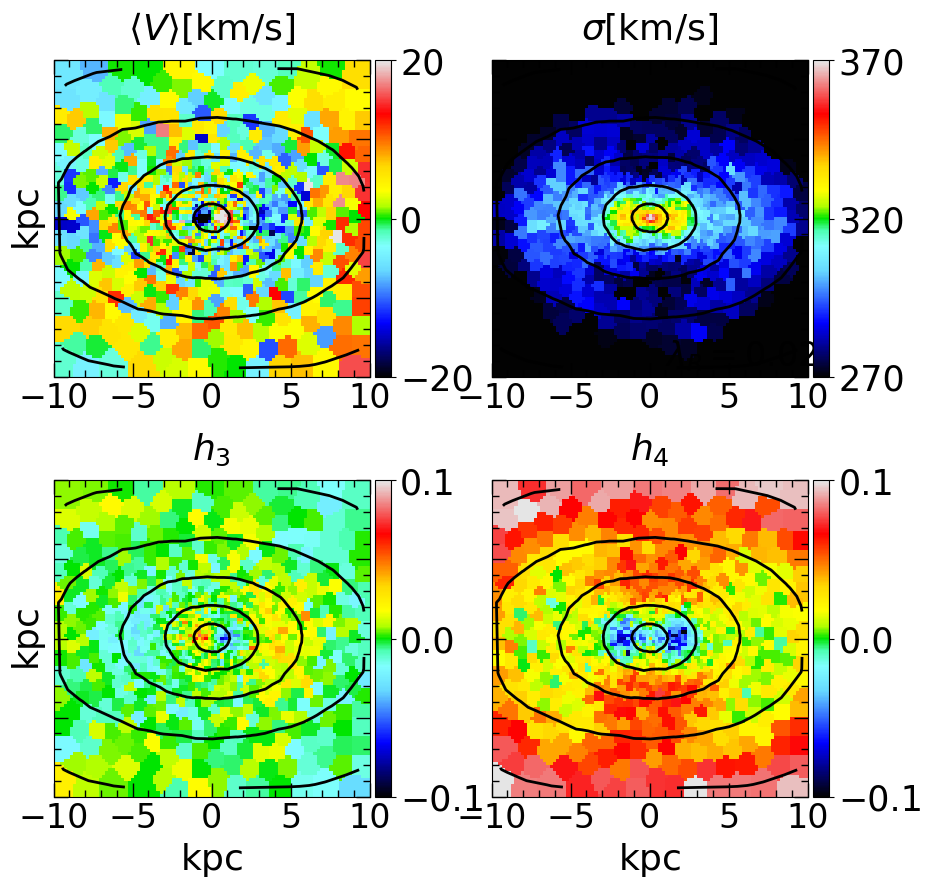
\includegraphics[width=\textwidth]{BH_5.png}
		\caption{BH-3 merger}
	\end{subfigure}
	\caption{IFU-maps of average LOS-velocities, velocity dispersion, $h_3$ parameters and $h_4$ parameters from four simulated merger remnants: BH-1, BH-2, BH-3, BH-4 and BH-5 mergers.}
	\label{figure:rest_of_voronoi}
\end{figure}


 %Furthermore, the velocity dispersion maps also show features found in observed galaxies (figure \ref{figure:IFU-maps}). \textit{Stuff about the features?}

Apart from the BH-0 merger remnant, the $h_3$-parameter values in the IFU-maps of the simulated merger remnants show an anti-correlation with the average LOS-velocity. Indeed, \cite{Krajnovic2011} have found that, while the anti-correlation between the LOS velocities and the $h_3$-parameter is mostly found in fast rotators, some galaxies with counter-rotating cores (CRC) also exhibit this behaviour. This anti-correlation can be seen in NGC 3414 from figure \ref{figure:IFU-maps}. Once again, the simulated KETJU results agree with the observations.

The $h_4$-parameter roughly corresponds to the velocity anisotropy parameter $\beta$, where a negative value of $h_4$ identifies areas with a large tangential velocity dispersion, and a positive identifies areas with a more radial velocity dispersion \citep{Gerhard1993, Gerhard1998, Thomas2007}. Comparing the $\beta$-profiles from figure \ref{figure:beta_no_rb} with the $h_4$ IFU-maps from figures \ref{figure:IFU-maps} and \ref{figure:rest_of_voronoi}, this certainly seems to be the case. For the merger remnants with central SMBH binaries, both the $\beta$ and the $h_4$ values are largely positive in the outer regions of the galaxy, while being negative closer to their centres. The $h_4$ map of the BH-0 merger is then positive all around, exactly like its $\beta$-profile. The $h_4$ maps of NGC 3414 and NGC 4111 (figure \ref{figure:IFU-maps}) do not contain any specific structures and seem to be completely isotropic. As the negative $h_4$-areas in the IFU maps of the simulated merger remnants are likely caused by core scouring, and as neither of the observed galaxies are cored galaxies \citep{Lauer2007}; they most likely have not experienced such a process, making the lack of clear structures understandable.

\subsection{The $\lambda_R$-parameter}

Further analysis on the kinematics of the simulated merger remnants can be done by studying the $\lambda_R$ parameter, which describes the angular momentum of a galaxy \citep{Emsellem2007}. More importantly, the parameter allows us to differentiate between the aforementioned slowly rotating galaxies and so-called fast rotators (see figure \ref{figure:IFU-maps}) \citep{Emsellem2007}. The parameter itself is defined in a general form as:
\begin{equation}
\lambda_R \equiv \frac{\langle R |V| \rangle}{\langle R \sqrt{V^2 + \sigma^2} \rangle}, \label{eq:general_lambdar}
\end{equation}
where $R$ is the projected distance from the galactic centre, $V$ is the line-of-sight velocity, $\sigma$ is the velocity dispersion and $\langle \; \rangle$ denote that the nominator and denominator in the equation are luminosity weighted means. However, as most of the observational kinematic analysis of galaxies is done through binned 2D spectroscopy, and as the IFU-maps made from our simulations are produced the same way as the observed ones, we will be using the following version of the equation:
\begin{equation}
\lambda_R = \frac{\sum^{N_p}_{i=1} F_i R_i |V_i|}{\sum^{N_p}_{i=1} F_i R_i \sqrt{V_i^2 + \sigma^2_i}}, \label{eq:binned_lambdar}
\end{equation}
where $F_i$, $R_i$, $V_i$ and $\sigma_i$ are the flux, projected distance from the galaxy centre, velocity and velocity dispersion of the $i$th bin, and $N_p$ is the number of bins. In the case of our simulations, the $N_p$ bins used are of course the voronoi bins described earlier in this section. 

Determining whether a galaxy is either a fast or a slow rotator using $\lambda_R$, is done by comparing the value that the parameter gets at the galaxy's effective radius, to some pre-defined threshold. The originally used threshold is: $\lambda_{Re} < 0.1$, where $\lambda_{Re}$ is the aforementioned $\lambda_R$ at the effective radius, and where galaxies fulfilling this condition are classified as slow rotators \citep{Emsellem2007}. A revision of the threshold by \cite{Emsellem2011} takes the ellipticity ($\epsilon$, defined in chapter 2) of the galaxy into account, and defines slow rotators as having $\lambda_{R_e} < 0.31 \sqrt{\epsilon}$, which accounts for the increased anisotropy in the kinematics of flatter galaxies. An even further refinement of the threshold has been proposed by \cite{Cappellari2016}, where slow rotator galaxies are determined using the following two criteria: $\lambda_{R_e} < 0.08 + \epsilon/4$ and $\epsilon < 0.4$. The former criterion of the threshold reduces the risk of misidentifying very round non-regular slow rotators as fast rotators, while the latter makes sure that only sufficiently round galaxies are classified as slow rotators (\cite{Cappellari2016} argues that "genuine" disk-less slow rotators are all rounder than $\epsilon = 0.4$).

Since two of the three aforementioned slow rotator thresholds require us to know the ellipticity of the galaxy, before analysing their rotation, I wrote a program in Python that calculates ellipticities of the simulated merger remnants. The ellipticity calculations are done using a method described in \cite{Zemp2011}, which uses the shape tensor:
\begin{equation}
\mathbf{S} = \frac{\int_V \rho(\mathbf{r}) \omega(\mathbf{r}) \mathbf{r} \mathbf{r}^T \; dV }{\int_V \rho{\mathbf{r}} \; dV},
\end{equation}
where $\mathbf{r}$ is position from the galactic centre, $\rho(\mathbf{r})$ is the mass density, $V$ is the volume of an enclosed ellipsoid with the elliptical radius $r_\mathrm{ell}$, and where the weighting function $\omega(\mathbf{r}) = 1$. The eigenvalues of the shape tensor correspond to $a^2/3$, $b^2/3$ and $c^2/3$; where $a$, $b$ and $c$ are the semi-principal axes; and which can be used to calculate the ellipticity as $\epsilon = 1 - b/a$. 

However, simply calculating the shape tensor and getting the correct eigenvalues is not possible, as the elliptical radius $r_\mathrm{ell}$ is defined, in part, by using the axis ratios $a/b$ and $a/c$:
\begin{equation}
r_\mathrm{ell} = \sqrt{x_\mathrm{ell}^2 + \frac{y_\mathrm{ell}^2}{(b/a)^2} + \frac{z_\mathrm{ell}^2}{(c/a)^2}}.
\end{equation}
This means that we have to turn the calculation into an iterative process by starting with $b/a = c/a = 1$ for the initial value of $r_\mathrm{ell}$, and calculating new shape tensor eigenvalues using previously gained axis ratios until the values of the ratios start to converge. 

We calculate $\lambda_{Re}$ and $\epsilon_e$, i.e. the ellipticity at the effective radius (the ellipticity is calculated using $r_\mathrm{ell} = R_e$, and a convergence criterion of a difference smaller than $10^{-3}$ between consequent axis ratios), for every merger simulation snapshot and plot them against each other. We also plot the previously mentioned slow rotator thresholds, as well as observations from the $\mathrm{ATLAS^{3D}}$-survey \citep{Cappellari2011}, in the same figure. The resulting plot can be seen in figure \ref{figure:lambda_epsilon}. 

\begin{figure}[h]
	\centering
	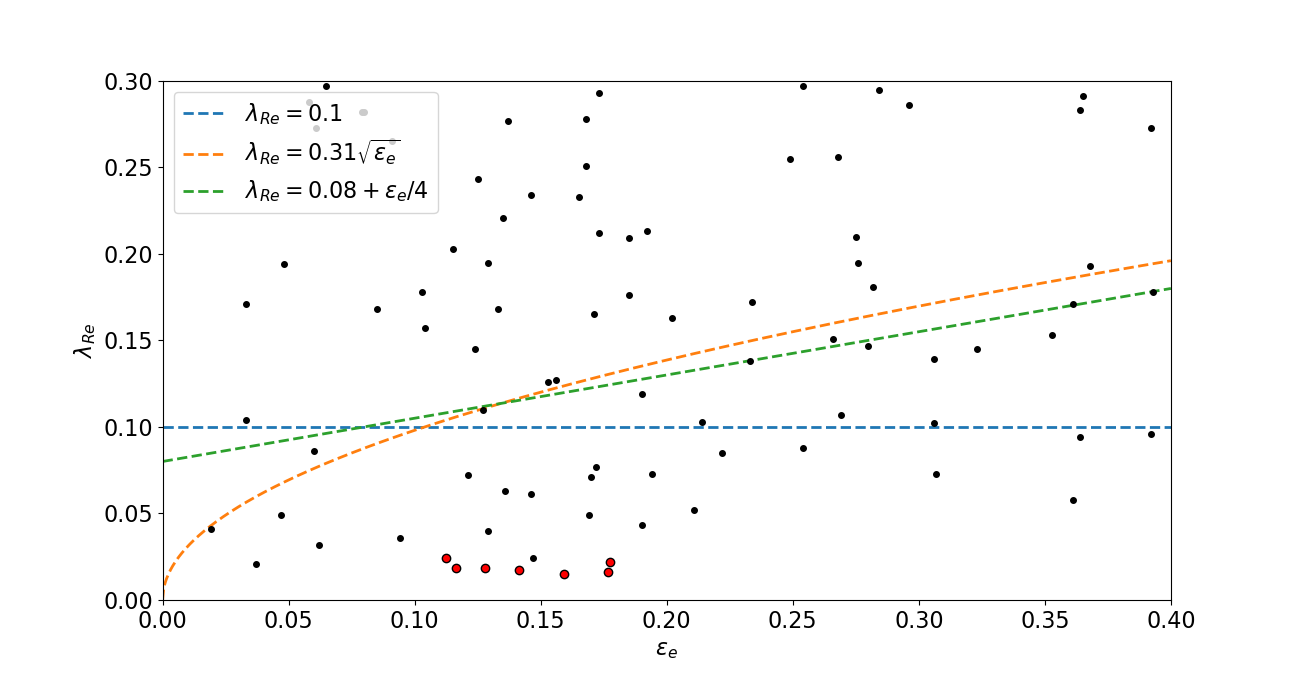
\includegraphics[width=\textwidth]{lambda_epsilon.png}
	\caption{The values of the $\lambda_{\mathrm{Re}}$-parameter of galaxies, plotted against their ellipticity at the effective radius. The red dots correspond to the simulated merger remnants, where as the black dots correspond to galaxies observed in the $\mathrm{ATLAS^{3D}}$-survey \citep{Cappellari2011, Emsellem2011}. The dashed lines display different slow rotator thresholds as a function of ellipticity \citep{Emsellem2007, Emsellem2011, Cappellari2016}.}
	\label{figure:lambda_epsilon}
\end{figure}

Regardless of the threshold used for differentiating between slow and fast rotators, figure \ref{figure:lambda_epsilon} shows us that, all of the simulated merger remnants are clearly classified as slow rotators. This agrees well with the kinematic anisotropies seen in the IFU maps, which also implied a slow rotator classification for the remnants.

\section{Comparison to Observations}

- BH-6, NGC 1600 samat kinemaattiset propertiit ja mu-profiilit. dry ETG merger tod.näk. muodstumismekanismi
- BH-1 samat kinematiikat. SMBH massa ei vaikuta kinematiikkaan, tod.näk vaan progenitoreiden muut ominaisuudet
- NGC 4472 eri kinematiikat. syntynyt eri tavalla? pitää ottaa huomioon lambdan epätarkkuus
- BH-1 ja NGC 4472 about sama core radius. vain SMBH massat vaikuttaa. voi tietty olla vaan sattumaa.

As the physical properties of the merger progenitors are modelled after NGC 1600, it is interesting to see how the results from the simulations compare with actual observations of the galaxy. I will be comparing the observations mainly to the BH-6 merger remnant, as the mass of the SMBH binary in the simulated galaxy is equivalent to the observed and modelled mass of the central SMBH in NGC 1600 ($M_\bullet = 1.7 \times 10^{10} M_\odot$) \citep{Thomas2016}. I will also be comparing the observed properties of the cored massive elliptical galaxy NGC 4472 to the simulated BH-1 merger remnant. Both of them have similar central black hole (or in the case of the simulated remnant, black hole binary) masses, as well as similar total stellar masses. Thus, comparing their other physical properties could provide some interesting insight into the formation of cores.

Figure \ref{figure:profile_comparison} shows core-Sérsic profile fits of the surface brightness profiles from the BH-1 and BH-6 mergers, and compares them to the profile fits from the observed core galaxies NGC 4472 and NGC 1600 respectively. Not only do the shapes of the compared profiles follow each other closely in both cases, the best-fit parameters are also quite closely related (table \ref{table:bestfit_parameter_comparison}). 

\begin{table}
	\begin{center}
		\scriptsize
		\begin{tabular}{| c | c c | c c |}
		\hline
		 & BH-1 merger & NGC 4472 & BH-6 merger & NGC 1600 \\
		\hline
		$r_b \; \mathrm{[kpc]}$ & $0.137$ & $0.151$ & $0.579$ & $0.667$ \\
		$\mu_b \; \mathrm{[mag \, arcsec^{-2}]}$ & $16.29$ & $16.48$ & $17.68$ & $18.00$ \\
		$R_e \; \mathrm{[kpc]}$ & $9.717$ & $16$ & $9.304$ & $16.04$ \\
		$n$ & $4$ & $5.6$ & $4$ & $5.83$ \\
		$\alpha$ & $1.45$ & $3.05$ & $1.22$ & $2.09$ \\
		$\gamma$ & $0.00$ & $0.06$ & $-0.04$ & $0.03$ \\
		\hline
		\end{tabular}
	\end{center}
	\caption{Best-fit parameters of the core-Sérsic profile fit seen in figure \ref{figure:profile_comparison}. The best-fit parameters of NGC 4472 are from \cite{Rusli2013}, while the parameters for NGC 1600 are given in \cite{Thomas2016}.}
	\label{table:bestfit_parameter_comparison}
\end{table}

Another comparison between some of the properties of the four galaxies can be seen in table \ref{table:snap6_vs_NGC1600}. Most importantly, the table shows that the kinematic properties of the simulated merger remnants and the kinematic properties of NGC 1600 are very similar. On the other hand, compared to the three other galaxies, the spin parameter and line-of-sight velocity of NGC 4472 are almost an order of magnitude larger. Furthermore, like the simulated galaxies, NGC 1600 can easily be identified as a slow rotator by its $\lambda_e$ parameter and ellipticity, while NGC 4472 seems to be classified as a fast rotator. 

Before drawing conclusion from these results, it is important to know that, whether NGC 4472 is in fact classified as a fast rotator is not known for certain. \cite{Emsellem2011} found a significantly lower value for its spin parameter ($\lambda_e = 0.077$), which would easily classify the object as a slow rotator. The value used in this analysis comes from the more recent MASSIVE-survey \citep{Ma2014MASSIVE, Veale2017veldisp}, in which some of the inaccuracies of the aforementioned calculations were shown (e.g. not taking into account a large enough region of the observed galaxy). Conceding to some possible biases in their own calculations, \cite{Veale2017veldisp} ultimately classify NGC 4472 as an intermediate case between slow and fast rotators.

It is impressive, that the simulation of the BH-6 merger is able to reproduce both the kinematic properties and the shape of the surface brightness profile of NGC 1600 so well. Since the simulation describes a dry merger event between two massive ETG with central SMBHs, the results imply that this process could be the formation mechanism behind core galaxies. 

Interestingly, since the BH-6 merger has extremely similar kinematic properties with the BH-1 merger and NGC 1600, it can be assumed that the mass of the central SMBH binary does not affect the rotation of its host galaxy in any significant way. This suggests that, as far as the merger progenitors are concerned, it is the properties other than their central SMBH mass (i.e. them being massive gas-poor ETGs) that determine the kinematic properties of the final merger remnant. As for NGC 4472, since both its $\lambda_e$ and LOS velocity are about an order of magnitude larger compared to the three other galaxies, it can be argued that its formation history must be quite different. However, due to the ambiguity of whether NGC 4472 is a fast rotator and whether its spin parameter is biased towards large values, the possibility that the galaxy has also formed through a dry ETG merger, should not be ruled out.

Earlier in this chapter it was discussed that there is a clear positive correlation between the central SMBH binary masses and the size of the core radii. However, the facts that the core radius sizes for the BH-1 merger remnant and NGC 4472 are comparable, and that many of their other properties are quite different; imply that, not only is there a correlation, the SMBH binary mass might be the only property that affects the size of the core in any significant way. If this is true, it is extremely clear evidence, that the cores are formed through a scouring process by binary SMBHs.


\begin{table}
	\begin{center}
		\scriptsize
		\begin{tabular}{c c c c c c c c c c}
		\hline
		\hline
		Galaxy & $M_\star$ & $M_\bullet$ & $R_e$ & $\mu_e$ & $n$ & 
		$V_\mathrm{LOS}$ & $\sigma_e$ & $\lambda_e$ &
		$\epsilon_e$ \\
		& $[\times 10^{11} M_\odot]$ & $[\times 10^{10} M_\odot]$ &
		[kpc] & [$\mathrm{mag/arcsec^2}$] & & [km/s] & [km/s] & & \\
		(1) & (2) & (3) & (4) & (5) & (6) & (7) & (8) & (9) & (10) \\
		\hline
		BH-6 merger & $8.3$ & $1.7$ & $10.722$ & $21.54$ & $4$ & $5.61$ & $278$ & $0.0213$ & $0.15$ \\
		NGC 1600 & $8.3$ & $1.7$ & $\sim 16$ & $\sim 22.8$ & $5.83$ & $7.1$ & $293$ & $0.026$ & $0.32$ \\
		\hdashline
		BH-1 merger & $8.3$ & $0.17$ & $9.879$ & $21.42$ & $4$ & $5.49$ & $274$ & $0.021$ & $0.195$ \\
		NGC 4472 & $6.03$ & $0.25$ & $14.33$ & $22.72$ & $5.6$ & $45.4$ & 
		$258$ & $0.197$ & $0.172$ \\
		\hline
		\end{tabular}
	\end{center}
	\caption{Comparisons between the physical properties of the simulated BH-1 and BH-6 merger remnants and the observed galaxies NGC 1600 and NGC 4472 respectively. The properties described in the columns are explained below, alongside the sources for the properties of NGC 1600 and NGC 4472. \\
	(1) Name of the galaxy. \\
	(2) Total stellar mass. NGC 1600: \cite{Thomas2016}, NGC 4472: \cite{Veale2018lambda}. \\
	(3) Central SMBH / central SMBH binary mass. NGC 1600:  \cite{Thomas2016}, NGC 4472: \cite{Rusli2013_BHmass}. \\
	(4) Effective radius. The values used for the simulated mergers are estimated by calculating the half-mass radius in three dimensions, and using equation \ref{eq:projection_approximation} to get the approximate two dimensional effective radius. This is done instead of using the core-Sérsic profile best-fit parameter, since the core-Sérsic $R_e$ only takes into account the specific fitting radius. NGC 1600: \cite{Thomas2016}, where the value is changed from arc seconds to kpc by assuming that the galaxy is located at the distance of $D = 64 \; \mathrm{Mpc}$; NGC 4472: \cite{Veale2017veldisp}. \\
	(5) Surface brightness at the effective radius. The values for all of the galaxies are calculated from the core-Sérsic fits. The profile fits best-fit parameters are from table \ref{table:bestfit_parameter_comparison}. \\
	(6) Sérsic index. NGC 1600: \cite{Thomas2016}, NGC 4472: \cite{Rusli2013}. \\
	(7) Mean line-of-sight velocity inside the effective radius. For the the simulated mergers these values are calculated from their respective IFU maps as the mean of the $V_{LOS}$-values from the Voronoi-bins inside the effective radius. NGC 1600 and NGC 4472: \cite{Bender1994}. \\
	(8) Velocity dispersion inside the effective radius. As with $V_{LOS}$, this value comes from the mean velocity dispersion of the Voronoi bins inside the effective radius in the IFU-maps of the simulated mergers. NGC 1600 and NGC 4472: \cite{Veale2017veldisp}.\\
	(9) Spin parameter at the effective radius. NGC 1600 and NGC 4472: \citep{Veale2018lambda}. \\
	(10) For the simulated mergers and NGC 4472: ellipticity of the galaxy at the effective radius. For NGC 1600: luminosity weighted ellipticity. NGC 1600: \cite{Goullaud2018}, NGC 4472: \cite{Emsellem2011}.
	}
	\label{table:snap6_vs_NGC1600}
\end{table}

\begin{figure}
	\centering
	\begin{subfigure}[b]{0.49\textwidth}
		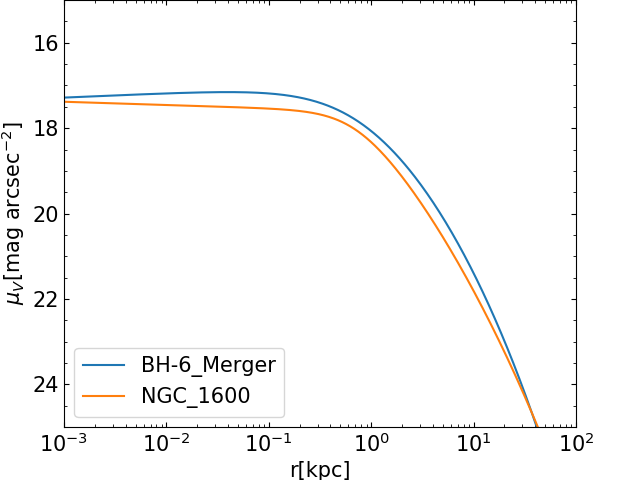
\includegraphics[width=\textwidth]{BH-6_NGC1600.png}
	\end{subfigure}
	\begin{subfigure}[b]{0.49\textwidth}
		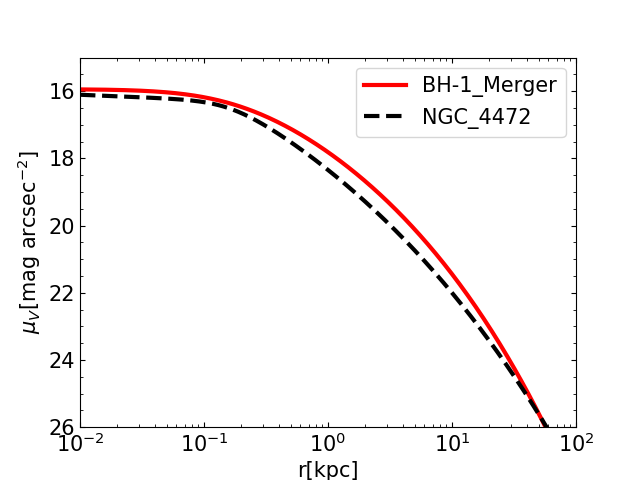
\includegraphics[width=\textwidth]{BH-1_NGC4472.png}
	\end{subfigure}
	\caption{Comparison between core-Sérsic profile fits from observed galaxies and simulated merger remnants, where the surface brightness is given in V-band magnitudes. The figure on the left compares the profile of the BH-6 merger remnant (the merger remnant whose progenitors containing the largest central SMBH massess) to NGC 1600; while the figure on the right compares the profiles of the BH-1 merger remnant (the remnant with progenitors that had the smallest SMBH masses) and NGC 4472. The parameters for plotting the core-Sérsic profile of NGC 1600 were taken from \cite{Thomas2016}, with the units being changed to the above, by assuming $V - R = 0.5$ (the same assumption being done in \cite{Lauer2007}), and by using the distance $D = 64 \mathrm{Mpc}$ \citep{Thomas2016} to define the relation between arc seconds and parsecs. The parameters for the profile of NGC 4472 were from \cite{Rusli2013}. All of the best-fit parameters can be found in table \ref{table:bestfit_parameter_comparison}}
	\label{figure:profile_comparison}
\end{figure}


\chapter{Conclusions}

\appendix

\chapter{Figures}

\begin{figure}
	\centering
	\begin{subfigure}[b]{0.49\textwidth}
		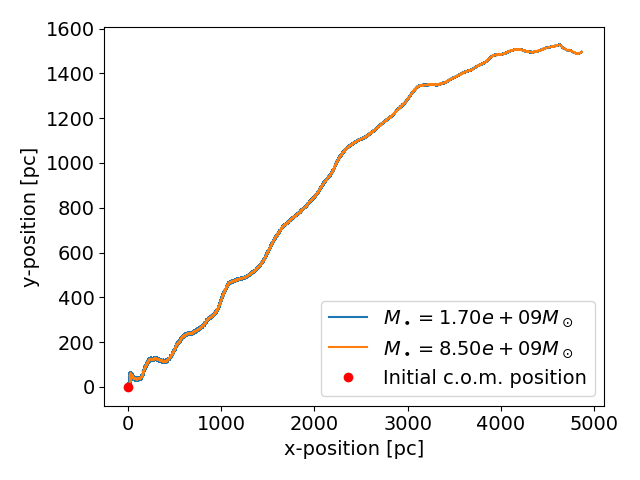
\includegraphics[width=\textwidth]{Run1_Trajectory_small.png}
		\caption{Run 1}
	\end{subfigure}
	\begin{subfigure}[b]{0.49\textwidth}
		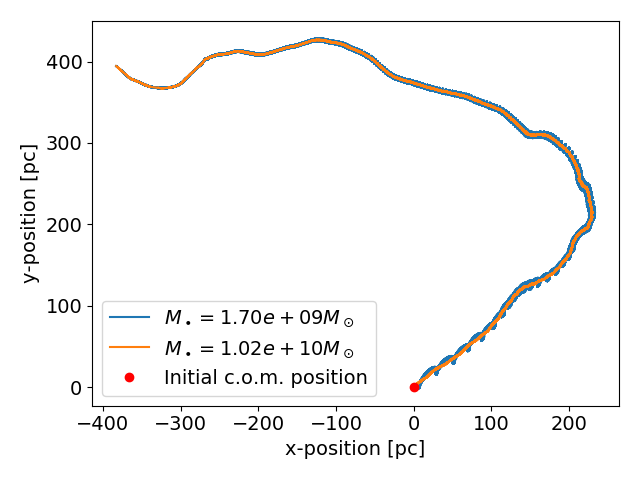
\includegraphics[width=\textwidth]{Run2_Trajectory_small.png}
		\caption{Run 2}
	\end{subfigure}
	\begin{subfigure}[b]{0.49\textwidth}
		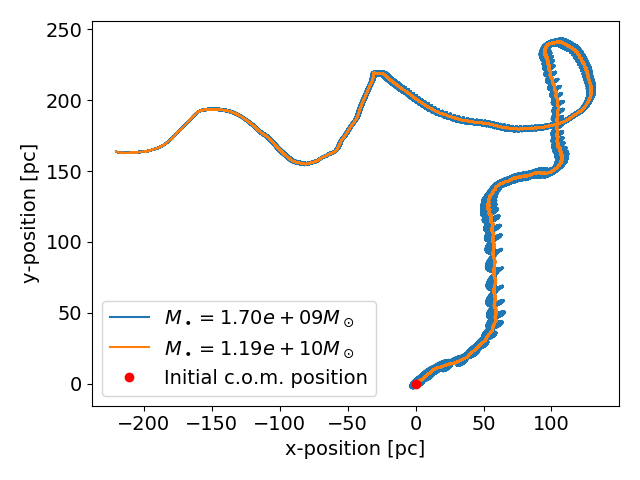
\includegraphics[width=\textwidth]{Run3_Trajectory_small.png}
		\caption{Run 3}
	\end{subfigure}
	\begin{subfigure}[b]{0.49\textwidth}
		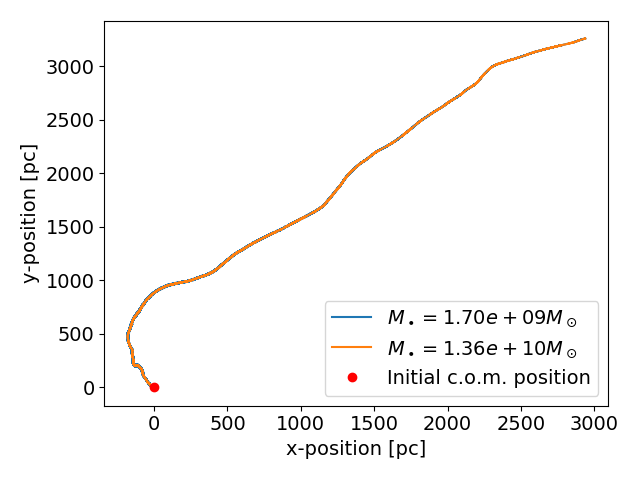
\includegraphics[width=\textwidth]{Run4_Trajectory_small.png}
		\caption{Run 4}
	\end{subfigure}
	\caption{The trajectories of the black holes from simulation runs by \cite{Mannerkoski2019}. The coordinates are centred on the initial location of the centre-of-mass of the black hole system. The orange and blue lines show the paths taken by the smaller and larger black holes respectively during the simulation.}
	\label{figure:all_traj}
\end{figure}

% STEP 5:
% Uncomment the following lines and set your .bib file and desired bibliography style
% to make a bibliography with BibTeX.
% Alternatively you can use the thebibliography environment if you want to add all
% references by hand.


% Define journal names
\newcommand{\apj}{The Astrophysical Journal}
\newcommand{\mnras}{Monthly Notices of the Royal Astronomical Society}
\newcommand{\apjs}{The Astrophysical Journal Supplement}
\newcommand{\nat}{Nature}
\newcommand{\aj}{The Astronomical Journal}
\newcommand{\na}{New Astronomy}
\newcommand{\araa}{Annual Review of Astronomy and Astrophysics}
\newcommand{\aap}{Astronomy and Astrophysics}
\newcommand{\apjl}{The Astrophysical Journal Letters}

\clearpage
\addcontentsline{toc}{chapter}{Bibliography} % This lines adds the bibliography to the ToC
\bibliographystyle{plainnat}
\bibliography{bibliography.bib}


\end{document}

